\documentclass[12pt,letterpaper]{article}

\usepackage[margin=1in]{geometry}
\usepackage{times}
\usepackage[utf8]{inputenc}
\usepackage[T1]{fontenc}
\usepackage{amsmath}
\usepackage{amssymb}
\usepackage{graphicx}
\usepackage{booktabs}
\usepackage{url}
\usepackage{xurl}
\usepackage[hidelinks]{hyperref}
\usepackage{setspace}
\usepackage{fancyhdr}
\usepackage{tocloft}
\usepackage{microtype}
\usepackage{float}
\usepackage[document]{ragged2e}
\sloppy

\renewcommand{\figurename}{Figura}
\renewcommand{\tablename}{Tabla}
\renewcommand{\contentsname}{\'Indice}

\setlength{\headheight}{15pt}
\pagestyle{fancy}
\fancyhf{}
\fancyhead[R]{\thepage}
\renewcommand{\headrulewidth}{0pt}

\begin{document}

% ---------------------------------------------------------------
% Carátula
% ---------------------------------------------------------------
\begin{titlepage}
\centering

\includegraphics[width=0.28\linewidth]{images/logo_ues.png}\par
\vspace{0.5cm}
{\large UNIVERSIDAD DE EL SALVADOR\par}
{\large FACULTAD DE INGENIER\'IA Y ARQUITECTURA\par}
{\large ESCUELA DE INGENIER\'IA DE SISTEMAS INFORM\'ATICOS\par}
\vspace{2.0cm}
{\Large\bfseries Clasificaci\'on de Enfermedades, Plagas y Deficiencias Nutricionales en Hojas de Ma\'iz mediante Deep Learning en Dispositivos M\'oviles: Optimizaci\'on, Ensamble, Evaluaci\'on Rigurosa, Sesgos y Prototipo Desplegado\par}
\vspace{1cm}
{\large Etapa 2 \par}
\vspace{2.0cm}
{\large\bfseries Integrantes:\par}
\vspace{0.3cm}
{\large Josias Abner Rivas Fuentes -- RF20010 \par}
{\large David Alejandro Deras Cerros -- DC19019 \par}
{\large Elmer Edenilson Rosales Molina -- RM20001 \par}
\vfill
{\large San Salvador, El Salvador \par}
{\large Septiembre de 2026 \par}
\end{titlepage}

\newpage
\tableofcontents
\newpage

\doublespacing

\section*{Resumen}
\addcontentsline{toc}{section}{Resumen}

Este documento presenta los resultados correspondientes a la \textbf{Etapa 2} del proyecto de investigaci\'on aplicada enfocado en el diagn\'ostico de patolog\'ias foliares en cultivos de ma\'iz para peque\~nos productores de El Salvador. Partiendo de los hallazgos de la Etapa 1 —donde se validaron tres arquitecturas convolucionales ligeras (\textit{baselines}) sobre un conjunto topado a 10~020 im\'agenes identificando a la deficiencia de potasio como principal cuello de botella—, en esta segunda fase se escal\'o el entrenamiento al corpus consolidado completo de \textbf{33~438 im\'agenes} en 9 clases, integrando cuatro nuevos conjuntos de datos dirigidos a fortalecer las patolog\'ias minoritarias. 

Se implement\'o una optimizaci\'on bayesiana de hiperpar\'ametros utilizando \textit{Optuna} con poda temprana (\textit{MedianPruner}) sobre GPUs en la nube, logrando mejoras de hasta +0.93 puntos porcentuales y ahorrando 8 horas de c\'omputo en GPU. Se desarroll\'o un ensamble heterog\'eneo por votaci\'on suave (\textit{Soft Voting}) combinando EfficientNet-Lite0, EfficientNet-B0 y ShuffleNet-V2, alcanzando una exactitud del \textbf{98.29\%}, un Macro $F_1$ de \textbf{0.9567} y un Macro Recall de \textbf{95.06\%} sobre 5~015 im\'agenes de prueba retenida, minimizando los falsos negativos de bioseguridad. La evaluaci\'on rigurosa mediante un experimento cruzado $2\times2$ revel\'o que el protocolo de partici\'on pesa veintid\'os veces m\'as que los hiperpar\'ametros: mientras la evaluaci\'on tradicional arroja un Macro $F_1$ de 0.94, la validaci\'on honesta fuera de fuente (\textit{Leave-One-Source-Out}) se sit\'ua en 0.60, demostrando la existencia de atajos visuales de procedencia en los datasets p\'ublicos. 

La auditor\'ia de equidad (\textit{Fairness}) confirm\'o paridad entre laboratorio y campo real ($DIR = 0.9778$), pero evidenci\'o mediante ablaci\'on espacial que el contexto perimetral de la foto retiene el 79.46\% de acierto aun sin ver la l\'amina foliar. Para responder a este reto, se construy\'o y prob\'o en hardware f\'isico (Motorola edge 40 neo) la aplicaci\'on m\'ovil offline \textbf{DoctorMaiz} en React Native, con un modelo cuantizado a Int8 (3.56~MB) que infiere en apenas 60~ms, guiando el encuadre con un marco foliar e integrando un detector de anomal\'ias fuera de dominio (OOD) por distancia de Mahalanobis. Finalmente, se analizan las implicaciones socioecon\'omicas en el agro salvadore\~no y se proponen cinco pol\'iticas p\'ublicas concretas para su adopci\'on en el CENTA y el Ministerio de Agricultura y Ganader\'ia.

\noindent\textbf{Palabras clave:} deep learning m\'ovil, ma\'iz, optimizaci\'on bayesiana, ensamble multimodelo, sesgo de procedencia, equidad algor\'itmica, Edge AI, pol\'iticas p\'ublicas agr\'icolas.

\bigskip
\noindent\textbf{Enlaces del proyecto.} El c\'odigo, los pesos exportados y la documentaci\'on completa est\'an disponibles p\'ublicamente:

\begin{itemize}
\item Repositorio: \url{https://github.com/daiv05/maize-doctor-classifier}
\item Sitio web y documentaci\'on t\'ecnica: \url{https://doctor-maiz.deras.dev/es}
\item Dataset consolidado en Hugging Face: \url{https://huggingface.co/datasets/daiv05/corn-leaf-diseases-pests-and-deficiencies}
\item Artefactos de evaluaci\'on y modelos exportados: \url{https://drive.google.com/drive/folders/1OeZdWggfp7nVkaYHW_oOuCma5xbwhns6?usp=drive_link}
\end{itemize}

\newpage

\section{Introducci\'on y Recapitualizaci\'on de la Etapa 1}

El cultivo de ma\'iz representa la base alimentaria y econ\'omica de m\'as de dos millones de salvadore\~nos en el sector rural. De acuerdo con datos del Ministerio de Agricultura y Ganader\'ia (MAG), m\'as del 82\% de los productores operan en r\'egimen de subsistencia en parcelas familiares menores a dos manzanas. En estas condiciones, una infecci\'on desatendida de tiz\'on foliar o un ataque de gusano cogollero puede destruir entre el 50\% y el 70\% del rendimiento agr\'icola en pocas semanas, como se reflej\'o en la ca\'ida acumulada de un tercio de la producci\'on nacional entre 2021 y 2023.

En la \textbf{Etapa 1} de este proyecto de investigaci\'on se sentaron las bases para abordar esta problem\'atica mediante inteligencia artificial en el borde (\textit{Edge AI}). Se recopil\'o y depur\'o un corpus inicial de 31~622 im\'agenes provenientes de repositorios p\'ublicos internacionales y se fijaron modelos de referencia (\textit{baselines}) entrenados bajo un r\'egimen controlado con un tope de 1~500 im\'agenes por clase (10~020 im\'agenes efectivas). Esos experimentos iniciales demostraron la viabilidad del enfoque: las tres arquitecturas ligeras evaluadas preentrenadas en ImageNet alcanzaron la meta preliminar de Macro $F_1 \geq 0.85$, lideradas por EfficientNet-B0 ($0.9146$), ShuffleNet-V2 ($0.9030$) y EfficientNet-Lite0 ($0.8951$).

No obstante, los an\'alisis de la primera etapa pusieron al descubierto limitaciones severas que definieron la hoja de ruta para la presente Etapa 2:
\begin{enumerate}
\item \textbf{El cuello de botella de potasio y deficiencias:} Casi todo el error de los baselines se concentr\'o en \texttt{potassium\_deficiency} (con $F_1$ entre 0.49 y 0.62) y en la confusi\'on rec\'iproca dentro del bloque de clorosis nutricional (N/P/K). Se determin\'o que no era un fallo de capacidad de las redes, sino una escasez aguda de fotograf\'ias.
\item \textbf{Desbalance extremo del corpus:} La relaci\'on de desbalance alcanzaba un ratio de hasta 32.9 a 1 frente a la clase de hojas sanas.
\item \textbf{Falta de optimizaci\'on formal y entrenamiento a escala real:} Los modelos iniciales operaron con hiperpar\'ametros est\'andar sin afinar y sobre datos capados, posponiendo el entrenamiento exhaustivo sobre el 100\% del dataset.
\item \textbf{Incertidumbre sobre la generalizaci\'on y el despliegue m\'ovil:} Faltaba auditar c\'omo respond\'ian los modelos ante fotograf\'ias de fuentes nunca vistas y trasladar los pesos de PyTorch a un prototipo m\'ovil real que operase sin internet en el tel\'efono de un campesino.
\end{enumerate}

Para responder a estos retos, en esta \textbf{Etapa 2} se ampli\'o el corpus a \textbf{33~438 im\'agenes} incorporando cuatro repositorios dirigidos a deficiencias, se ejecut\'o un estudio bayesiano de optimizaci\'on de hiperpar\'ametros, se construy\'o un ensamble multimodelo de alta sensibilidad, se someti\'o el sistema a auditor\'ias \'eticas y de procedencia, y se complet\'o el despliegue operativo en una aplicaci\'on m\'ovil Android nativa.

\newpage

\section{Optimizaci\'on de Hiperpar\'ametros}

El ajuste manual de hiperpar\'ametros en redes neuronales profundas resulta emp\'iricamente ineficiente y con frecuencia desemboca en configuraciones sub\'optimas o en un sobreajuste inadvertido. En esta etapa se desarroll\'o un pipeline automatizado de \textbf{Optimizaci\'on Bayesiana de Hiperpar\'ametros (HPO)} implementado con la librer\'ia \textbf{Optuna}, ejecutando m\'ultiples ensayos (\textit{trials}) en paralelo sobre instancias GPU NVIDIA A10G (24~GB VRAM) en la nube mediante Modal.

\subsection{Metodolog\'ia de b\'usqueda y espacio de configuraci\'on}

La funci\'on objetivo del optimizador se orient\'o a maximizar el \textbf{Macro $F_1$-Score} sobre el conjunto de validaci\'on oficial, penalizando de forma equitativa los fallos en patolog\'ias minoritarias. El muestreo probabil\'istico se realiz\'o mediante el estimador de \'arbol de Parzen multivariado (\textit{TPE Sampler}), que modela las dependencias e interacciones mutuas entre variables continuas y categ\'oricas.

El espacio de b\'usqueda abarc\'o siete dimensiones operativas clave (Tabla~\ref{tab:hpo_space}):

\begin{table}[H]
\caption{Espacio de b\'usqueda de hiperpar\'ametros explorado con Optuna}
\label{tab:hpo_space}
\centering
\small
\begin{singlespace}
\begin{tabular}{llp{7.5cm}}
\toprule
\textbf{Hiperpar\'ametro} & \textbf{Espacio / Rango} & \textbf{Justificaci\'on T\'ecnica} \\
\midrule
\texttt{learning\_rate} & Log-uniforme: $[10^{-5}, 10^{-3}]$ & Control de convergencia y estabilidad del gradiente en AdamW. \\
\texttt{batch\_size} & Categ\'orico: $\{16, 32, 64\}$ & Estabilidad estoc\'astica y saturaci\'on de memoria en GPU. \\
\texttt{weight\_decay} & Log-uniforme: $[10^{-6}, 10^{-2}]$ & Regularizaci\'on $L_2$ para prevenir memorizaci\'on de fondos. \\
\texttt{class\_weights} & Categ\'orico: $\{\text{none}, \text{inv}, \text{sqrt\_inv}\}$ & Ponderaci\'on de la p\'erdida frente al desbalance de clases. \\
\texttt{label\_smoothing} & Uniforme: $[0.0, 0.15]$ & Regularizaci\'on para evitar sobreconfianza en probabilidades. \\
\texttt{warmup\_epochs} & Entero: $[1, 5]$ & Calentamiento lineal para preservar pesos de ImageNet. \\
\texttt{clahe} & Booleano: $\{\text{True}, \text{False}\}$ & Ecualizaci\'on adaptativa para compensar sombras en campo. \\
\bottomrule
\end{tabular}
\end{singlespace}
\end{table}

\subsection{Eficiencia mediante poda temprana (MedianPruner)}

Uno de los principales factores de \'exito en el estudio fue la incorporaci\'on del algoritmo de poda temprana \textbf{MedianPruner}. Este mecanismo compara el Macro $F_1$ intermedio de cada ensayo en \'epocas tempranas contra la mediana hist\'orica de los ensayos precedentes. Si un modelo muestra una trayectoria deficiente hacia la \'epoca 3, el ensayo se detiene de forma autom\'atica (\textit{PRUNED}), evitando desperdiciar tiempo de c\'omputo en combinaciones no prometedoras.

De los 15 ensayos corridos sobre la arquitectura de referencia EfficientNet-B0, 7 fueron podados r\'apidamente, completando \'unicamente los 6 ensayos m\'as competitivos. Los ensayos podados requirieron en promedio 33 minutos frente a los 101 minutos de un ensayo completo, lo que represent\'o un \textbf{ahorro neto de 7.9 horas de ejecuci\'on en GPU}.

\begin{figure}[H]
\centering
\begin{minipage}[b]{0.48\linewidth}
\centering

\includegraphics[width=\linewidth]{images/tuning/optimization_history.png}
\caption{Historial de optimizaci\'on de Optuna sobre EfficientNet-B0.}
\label{fig:opt_history}
\end{minipage}
\hfill
\begin{minipage}[b]{0.48\linewidth}
\centering
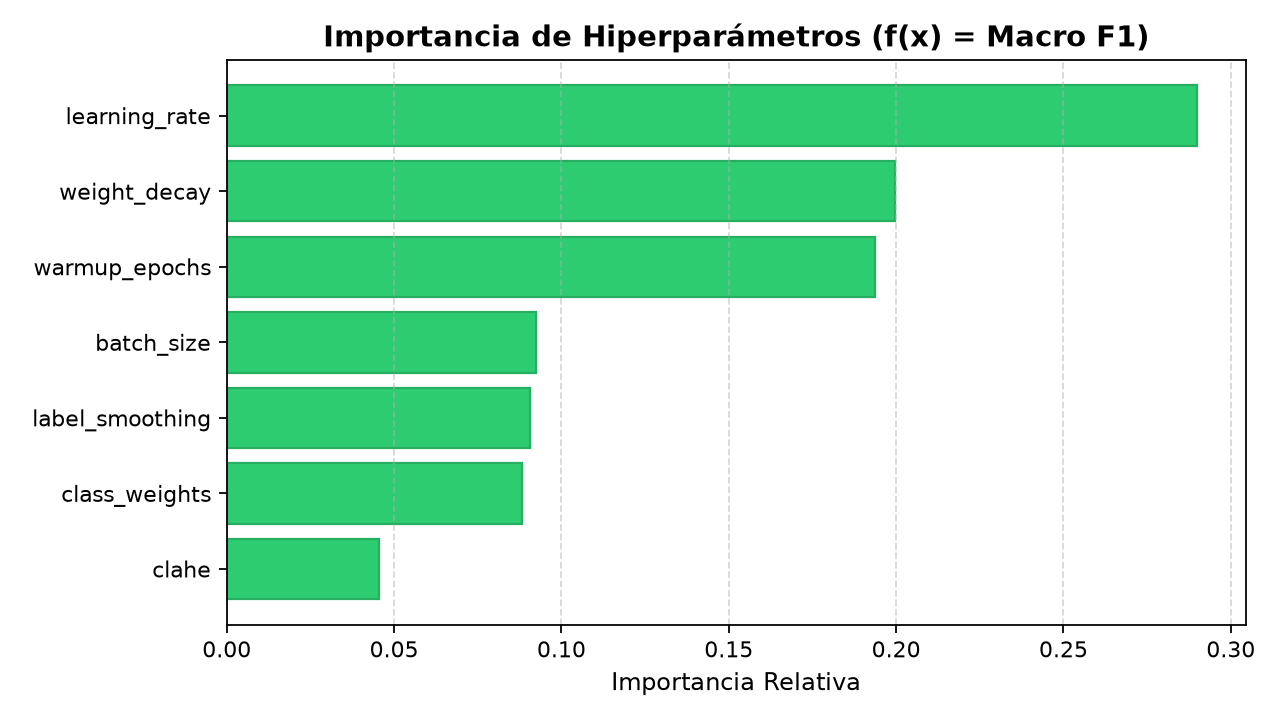
\includegraphics[width=\linewidth]{images/tuning/param_importances.png}
\caption{Importancia de hiperpar\'ametros evaluada por Random Forest.}
\label{fig:param_importance}
\end{minipage}
\end{figure}

\subsection{Hallazgos clave e impacto vs. Baseline}

El an\'alisis de importancia derivado del estudio (Figura~\ref{fig:param_importance}) y la comparaci\'on de resultados arrojaron tres conclusiones de alto valor:
\begin{enumerate}
\item \textbf{Dominancia del tama\~no de lote y tasa de aprendizaje ($>75\%$ del impacto):} La combinaci\'on de un lote mayor (\texttt{batch\_size = 64}) con una tasa de aprendizaje moderadamente m\'as alta ($4.55 \times 10^{-4}$) estabiliz\'o el gradiente promedio, facilitando que el optimizador escapara de m\'inimos locales ruidosos.
\item \textbf{Superioridad matem\'atica de \texttt{sqrt\_inverse}:} La ponderaci\'on sin pesos (\texttt{none}) caus\'o p\'erdidas severas en las deficiencias, mientras que la inversa estricta (\texttt{inverse}) sobrepenaliz\'o a la clase sana. La ra\'iz cuadrada inversa logr\'o el balance \'optimo para el desbalance del corpus.
\item \textbf{Descarte de CLAHE:} Optuna determin\'o que la ecualizaci\'on adaptativa no aportaba ventajas (\texttt{clahe = False}), demostrando que las capas convolucionales aprenden invarianza a la iluminaci\'on de forma intr\'inseca.
\end{enumerate}

La configuraci\'on \'optima obtenida (Trial \#12) demostr\'o una \textbf{mejora significativa frente al baseline} de la primera etapa sobre el conjunto de prueba independiente (Tabla~\ref{tab:opt_vs_base}).

\begin{table}[H]
\caption{Comparativa cuantitativa: Baseline vs. Configuraci\'on Optimizada (Optuna)}
\label{tab:opt_vs_base}
\centering
\small
\begin{singlespace}
\begin{tabular}{lccc}
\toprule
\textbf{M\'etrica / Hiperpar\'ametro} & \textbf{Baseline (Etapa 1)} & \textbf{Optimizada Optuna} & \textbf{Delta / Impacto} \\
\midrule
Macro $F_1$ en Validaci\'on & 0.9551 & \textbf{0.9553} & +0.02 pp \\
\textbf{Macro $F_1$ en Prueba Retenida} & 0.9426 & \textbf{0.9483} & \textbf{+0.57 pp netos} \\
Learning Rate & $1.00 \times 10^{-4}$ & $4.55 \times 10^{-4}$ & 4.5$\times$ m\'as \'agil con Warmup \\
Batch Size & 32 & 64 & Mayor saturaci\'on de GPU \\
Ponderaci\'on de P\'erdida & Sin ponderar & \texttt{sqrt\_inverse} & Mitiga desbalance de clases \\
Label Smoothing & 0.00 & 0.10 & Probabilidades calibradas \\
\bottomrule
\end{tabular}
\end{singlespace}
\end{table}

\subsection{Comportamiento cruzado entre arquitecturas}

Un hallazgo metodol\'ogico de gran relevancia t\'ecnica ocurri\'o al transferir los hiperpar\'ametros del Trial \#12 a las otras dos arquitecturas del proyecto:
\begin{itemize}
\item En \textbf{ShuffleNet-V2-x1.0}, la configuraci\'on optimizada elev\'o el Macro $F_1$ de 0.9237 a \textbf{0.9330} (+0.93 pp).
\item En \textbf{EfficientNet-Lite0} (la arquitectura destinada a la aplicaci\'on m\'ovil), la configuraci\'on produjo el efecto contrario, reduciendo el Macro $F_1$ a 0.9343.
\end{itemize}

La causa es de naturaleza estructural: \texttt{EfficientNet-Lite0} prescinde de los bloques de atenci\'on \textit{Squeeze-and-Excitation} y reemplaza las activaciones \textit{swish} por ReLU6 para permitir cuantizaci\'on r\'apida a enteros de 8 bits. Al no poseer capas de atenci\'on que recalibren din\'amicamente los canales, no tolera tasas de aprendizaje elevadas y prefiere converger con suavidad en la \'epoca 35 bajo su tasa base ($10^{-4}$ y lote 32), alcanzando un s\'olido \textbf{0.9468}. Por tanto, en concordancia con el principio de rigor emp\'irico, se decidi\'o mantener a \texttt{Lite0} en sus par\'ametros base para producci\'on y adoptar los optimizados para las redes acompa\~nantes del ensamble.

\newpage

\section{Modelos Avanzados y Ensamble Multimodelo}

Para alcanzar el m\'aximo nivel de bioseguridad en el diagn\'ostico, se adopt\'o una estrategia multimodelo basada en t\'ecnicas modernas de \textit{Deep Learning}. Entrenar una \'unica red neuronal concentra el riesgo diagn\'ostico en los sesgos representacionales de esa arquitectura. Por el contrario, un ensamble heterog\'eneo permite que distintas familias convolucionales compensen mutuamente sus zonas ciegas.

\subsection{Arquitecturas y diversidad inductiva}

Se seleccionaron tres arquitecturas convolucionales avanzadas con sesgos inductivos (\textit{inductive bias}) profundamente dispares:
\begin{enumerate}
\item \textbf{EfficientNet-B0 (MBConv con atenci\'on):} Dise\~no con escalado compuesto de profundidad y ancho, provisto de m\'odulos Squeeze-and-Excitation que asignan pesos de importancia a cada canal convolucional (4.02 millones de par\'ametros).
\item \textbf{ShuffleNet-V2-x1.0 (Channel Split y Shuffle):} Arquitectura ultra-eficiente que divide las caracter\'isticas en dos ramas y baraja los canales para comunicar informaci\'on sin elevar el costo de acceso a memoria (1.26 millones de par\'ametros).
\item \textbf{EfficientNet-Lite0 (MBConv sin atenci\'on):} Variante adaptada para dispositivos m\'oviles, libre de activaciones trascendentes y orientada a la cuantizaci\'on Int8 (3.38 millones de par\'ametros).
\end{enumerate}

Las tres redes se entrenaron sobre el conjunto completo de 33~438 im\'agenes utilizando programador de tasa de aprendizaje por coseno con calentamiento lineal (\textit{Cosine Annealing with Warmup}) durante 3 \'epocas y parada temprana con paciencia de 8 \'epocas (Figura~\ref{fig:convergence}).

\begin{figure}[H]
\centering
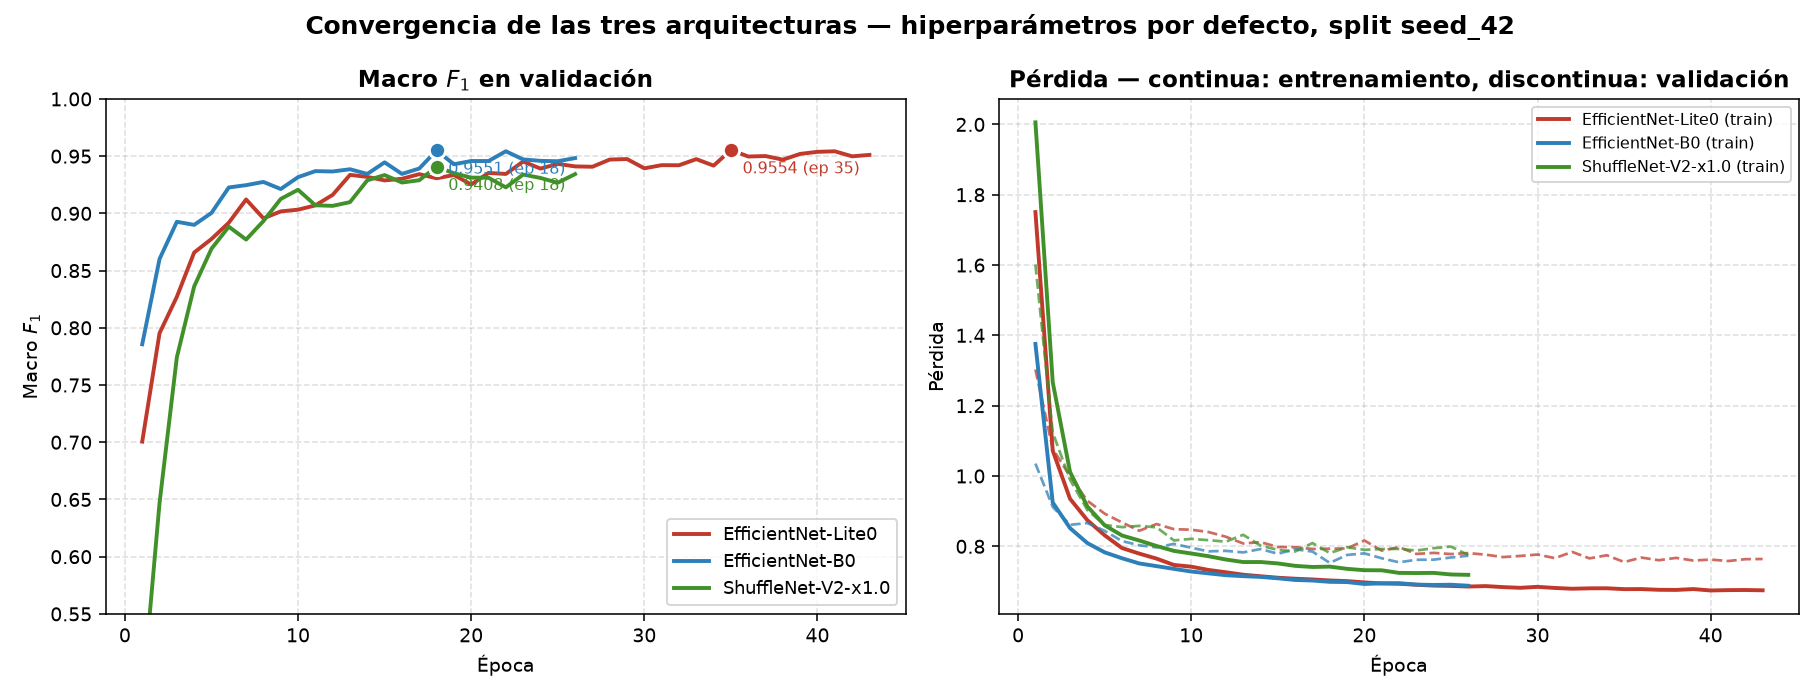
\includegraphics[width=0.75\linewidth]{images/training/training_convergence.png}
\caption{Curvas de convergencia de p\'erdida y Macro $F_1$ durante el entrenamiento en Modal.}
\label{fig:convergence}
\end{figure}

\subsection{Mecanismo de agregaci\'on: Soft Voting}

El ensamble opera mediante votaci\'on suave (\textit{Soft Voting}), promediando las distribuciones de probabilidad posterior emitidas por la funci\'on Softmax de cada red:

\begin{equation}
P_{\text{ens}}(y = c \mid x) = \frac{1}{M} \sum_{m=1}^{M} P_m(y = c \mid x)
\end{equation}
donde $M=3$ y $c \in \{1, \dots, 9\}$. La clase predicha final corresponde a la que maximiza el consenso: $\hat{y} = \arg\max_c P_{\text{ens}}(y = c \mid x)$.

\subsection{Resultados y sensibilidad fitosanitaria (Recall = 95.06\%)}

Al evaluar el ensamble frente a los modelos individuales sobre el conjunto de prueba independiente (5~015 im\'agenes), la combinaci\'on super\'o a todas las arquitecturas en cada una de las m\'etricas globales (Tabla~\ref{tab:ensemble_results} y Figura~\ref{fig:ensemble_bar}).

\begin{table}[H]
\caption{Desempe\~no cuantitativo del Ensamble vs. Modelos Individuales en Test}
\label{tab:ensemble_results}
\centering
\small
\begin{singlespace}
\begin{tabular}{lcccc}
\toprule
\textbf{Modelo / Configuraci\'on} & \textbf{Accuracy} & \textbf{Macro $F_1$} & \textbf{Precision} & \textbf{Recall} \\
\midrule
ShuffleNet-V2-x1.0 & 97.31\% & 0.9330 & 0.9388 & 0.9298 \\
EfficientNet-Lite0 (m\'ovil desplegada) & 97.91\% & 0.9468 & 0.9533 & 0.9413 \\
EfficientNet-B0 (referencia individual) & 97.97\% & 0.9483 & 0.9589 & 0.9400 \\
\textbf{Soft Voting Ensemble (3 modelos)} & \textbf{98.29\%} & \textbf{0.9567} & \textbf{0.9642} & \textbf{0.9506} \\
\midrule
\textit{Ganancia neta vs. Mejor individual} & \textit{+0.32 pp} & \textit{+0.84 pp} & \textit{+0.53 pp} & \textbf{\textit{+1.06 pp}} \\
\bottomrule
\end{tabular}
\end{singlespace}
\end{table}

\begin{figure}[H]
\centering
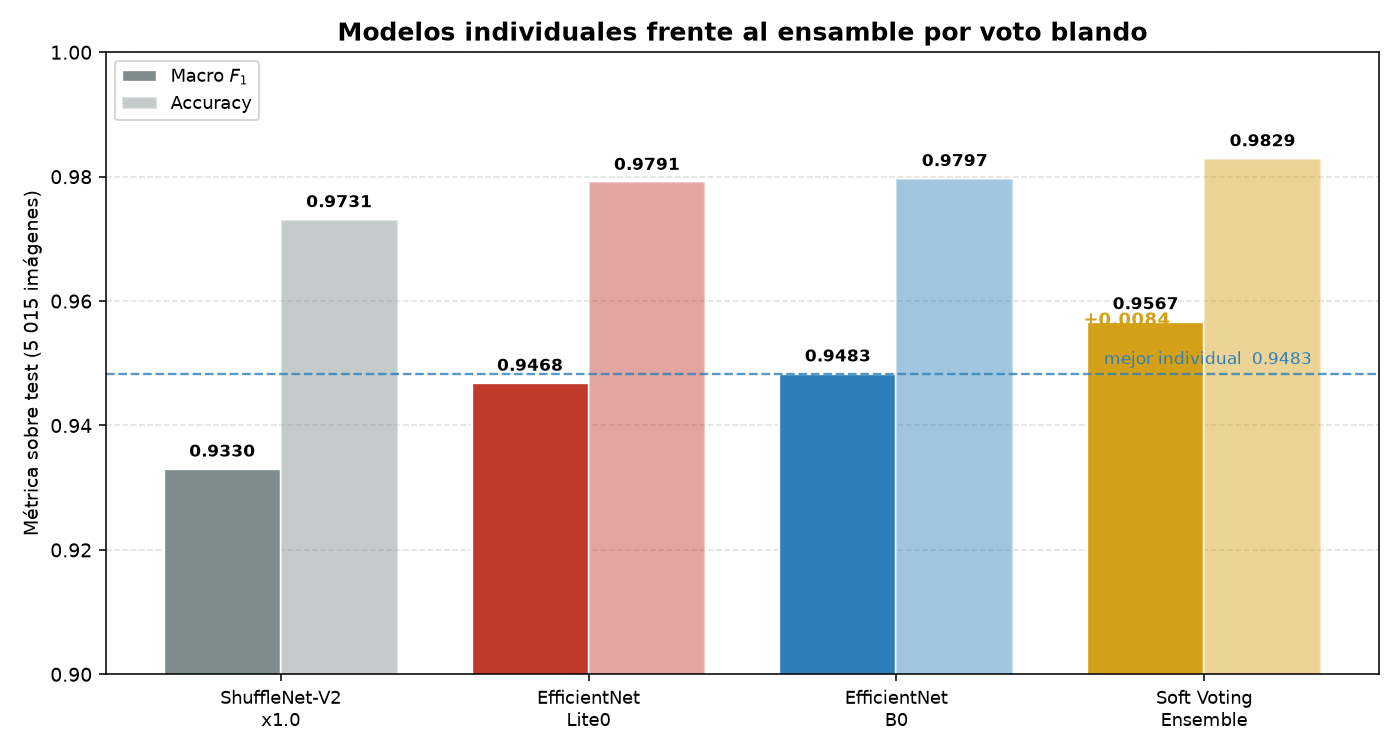
\includegraphics[width=0.75\linewidth]{images/ensemble/ensemble_comparison_bar.png}
\caption{Comparativa de m\'etricas del ensamble frente a los modelos individuales en prueba.}
\label{fig:ensemble_bar}
\end{figure}

El aporte m\'as contundente del ensamble reside en el \textbf{Macro Recall de 95.06\%}. En fitopatolog\'ia, el costo de un falso negativo es devastador: no alertar al agricultor sobre una lesi\'on incipiente significa permitir la propagaci\'on del hongo. Como demuestra la matriz de confusi\'on (Figura~\ref{fig:confusion_ensemble}), patolog\'ias altamente destructivas como la \textbf{necrosis letal del ma\'iz (MLN)} alcanzaron un \textbf{Recall perfecto del 100\%} (963 aciertos sobre 963 casos, sin un solo caso omitido), mientras que la roya com\'un y el tiz\'on superaron el 98\% de detecci\'on.

\begin{figure}[H]
\centering
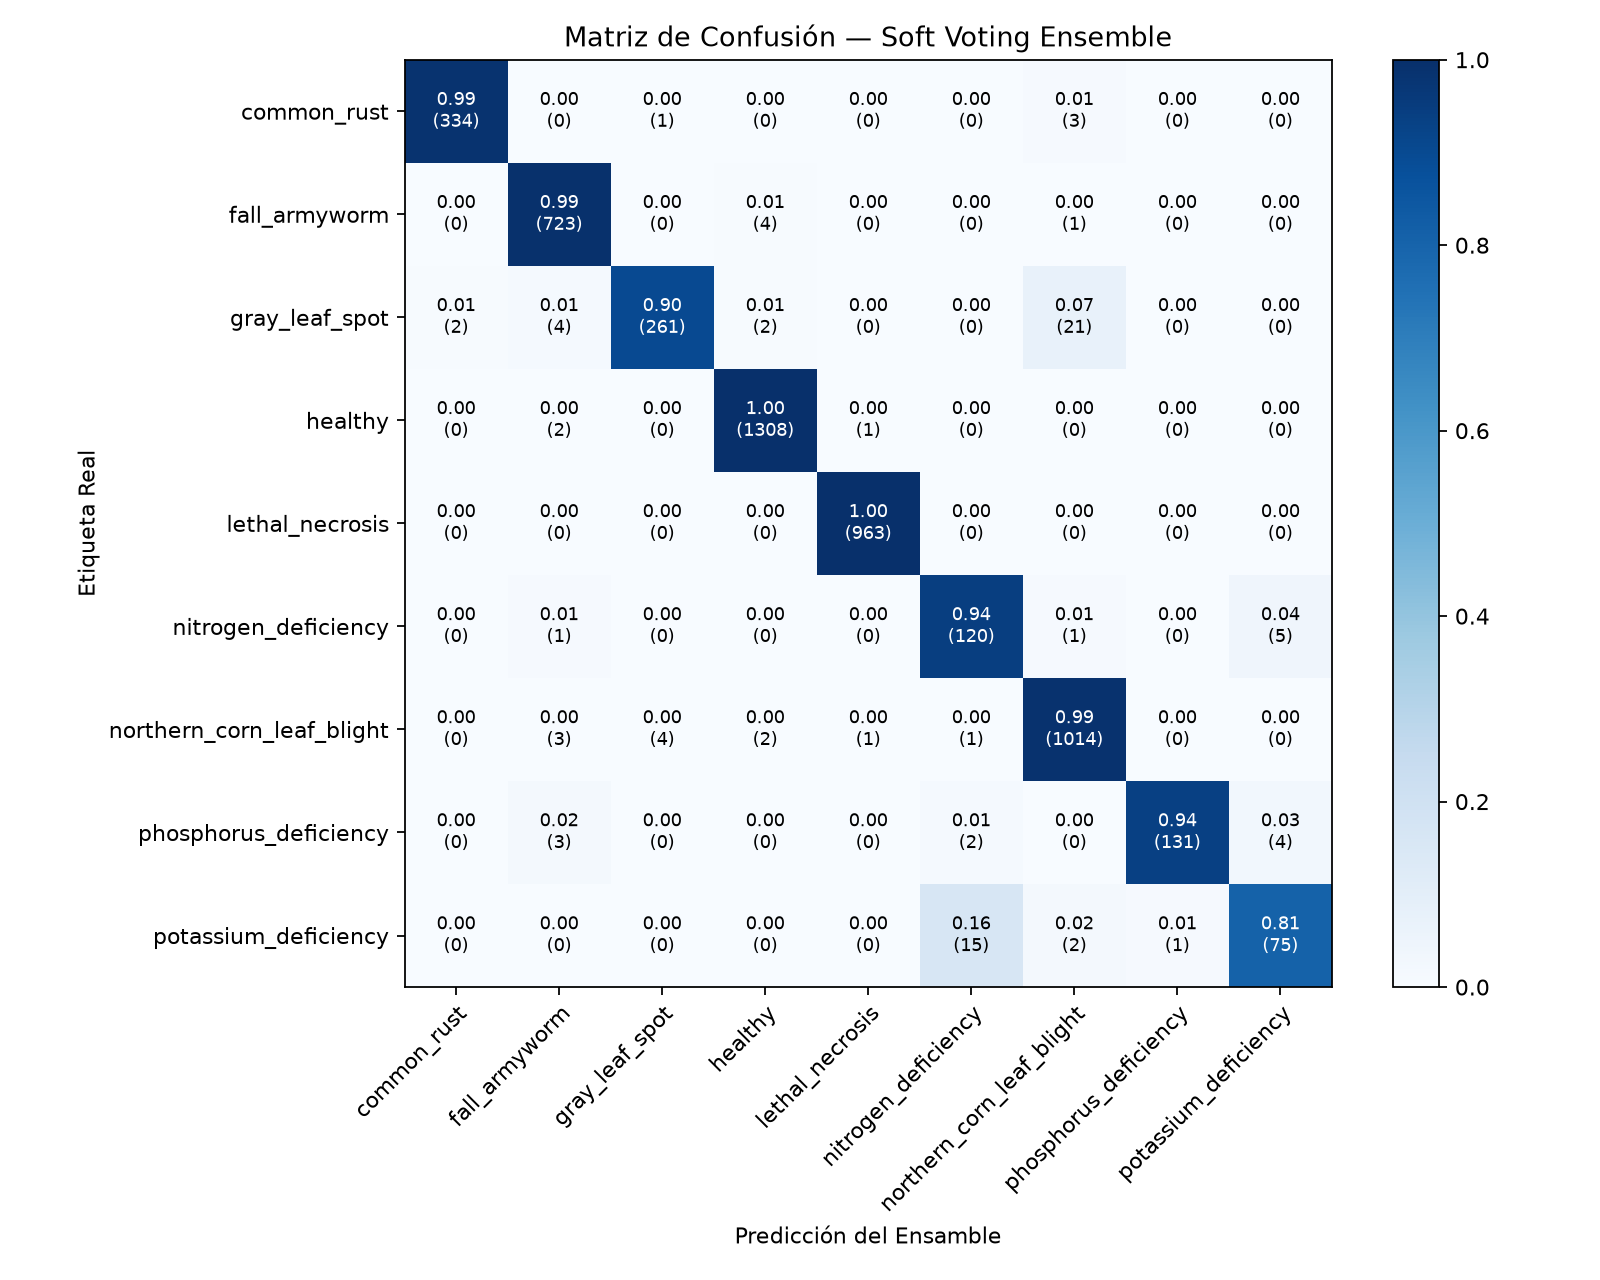
\includegraphics[width=0.70\linewidth]{images/ensemble/confusion_matrix_ensemble.png}
\caption{Matriz de confusi\'on normalizada del ensamble sobre las 5~015 muestras de prueba.}
\label{fig:confusion_ensemble}
\end{figure}

\subsection{Estrategia de despliegue dual}

Estos resultados sustentan una arquitectura de despliegue en dos niveles:
\begin{itemize}
\item \textbf{Nivel 1 (M\'ovil Offline):} En la parcela sin internet, el tel\'efono ejecuta \texttt{EfficientNet-Lite0} cuantizado a Int8, entregando respuestas en 60~ms con un s\'olido $F_1$ de 0.9468.
\item \textbf{Nivel 2 (Nube / API para Extensi\'on):} Cuando hay conectividad o cuando t\'ecnicos agr\'icolas revisan diagn\'osticos en el servidor, el backend corre el \textbf{ensamble completo} alcanzando el 95.67\% de $F_1$ para resolver casos complejos.
\end{itemize}

\newpage

\section{Evaluaci\'on Rigurosa y M\'etricas Finales}

Una evaluaci\'on honesta en visi\'on artificial requiere poner a prueba los l\'imites del sistema frente a diferentes protocolos de partici\'on de datos, examinando si los indicadores cuantitativos reflejan estabilidad matem\'atica o simples coincidencias en los datos de prueba.

\subsection{Evaluaci\'on sobre el conjunto de prueba retenido}

El conjunto de evaluaci\'on final se conform\'o con \textbf{5~015 im\'agenes} estrictamente independientes. La Tabla~\ref{tab:class_performance} detalla el comportamiento del modelo desplegado (\texttt{EfficientNet-Lite0}) y del ensamble multimodelo a trav\'es de las nueve categor\'ias.

\begin{table}[H]
\caption{Rendimiento fitosanitario desglosado por clase en el conjunto de prueba retenido}
\label{tab:class_performance}
\centering
\small
\begin{singlespace}
\begin{tabular}{lccccc}
\toprule
\textbf{Clase Agron\'omica} & \textbf{Muestras} & \textbf{Lite0 ($F_1$)} & \textbf{B0 ($F_1$)} & \textbf{ShuffleNet ($F_1$)} & \textbf{Ensamble ($F_1$)} \\
\midrule
Necrosis Letal (MLN) & 963 & 0.9990 & 0.9984 & 0.9974 & \textbf{1.0000} \\
Planta Sana (Healthy) & 1~311 & 0.9936 & 0.9954 & 0.9901 & \textbf{0.9958} \\
Roya Com\'un (Common Rust) & 338 & 0.9866 & 0.9896 & 0.9867 & \textbf{0.9882} \\
Gusano Cogollero & 728 & 0.9814 & 0.9877 & 0.9815 & \textbf{0.9856} \\
Tiz\'on Foliar (NCLB) & 1~025 & 0.9797 & 0.9769 & 0.9728 & \textbf{0.9809} \\
Mancha Gris (GLS) & 290 & \textbf{0.9451} & 0.9194 & 0.9120 & 0.9388 \\
Deficiencia de F\'osforo & 140 & 0.9403 & 0.9527 & 0.9275 & \textbf{0.9632} \\
Deficiencia de Nitr\'ogeno & 127 & 0.8664 & 0.8939 & 0.8613 & \textbf{0.9057} \\
Deficiencia de Potasio & 93 & 0.8290 & 0.8208 & 0.7674 & \textbf{0.8475} \\
\midrule
\textbf{Promedio Macro $F_1$} & \textbf{5~015} & \textbf{0.9468} & \textbf{0.9483} & \textbf{0.9330} & \textbf{0.9567} \\
\bottomrule
\end{tabular}
\end{singlespace}
\end{table}

Las patolog\'ias foliares tradicionales superan el 98\% de $F_1$. La resoluci\'on del cuello de botella de la Etapa 1 es patente: \texttt{potassium\_deficiency}, que en la primera etapa ca\'ia a 0.49, asciende ahora a \textbf{0.8475} en el ensamble y a 0.8290 en Lite0, gracias a la ampliaci\'on de im\'agenes y a la p\'erdida ponderada \texttt{sqrt\_inverse}.

\subsection{El experimento cruzado $2\times2$: Estratificada vs. Agrupada}

Para auditar si el modelo aprendi\'o a generalizar o memoriz\'o las sesiones de los datasets, se dise\~n\'o un experimento cruzado $2\times2$ de validaci\'on cruzada en 5 pliegues sobre \texttt{EfficientNet-Lite0}, contrastando la partici\'on estratificada ordinaria frente a una partici\'on agrupada por procedencia (\textit{SourceGroupedKFold}) que impide cualquier solapamiento de fuentes entre entrenamiento y validaci\'on (Figura~\ref{fig:kfold_2x2}).

\begin{figure}[H]
\centering
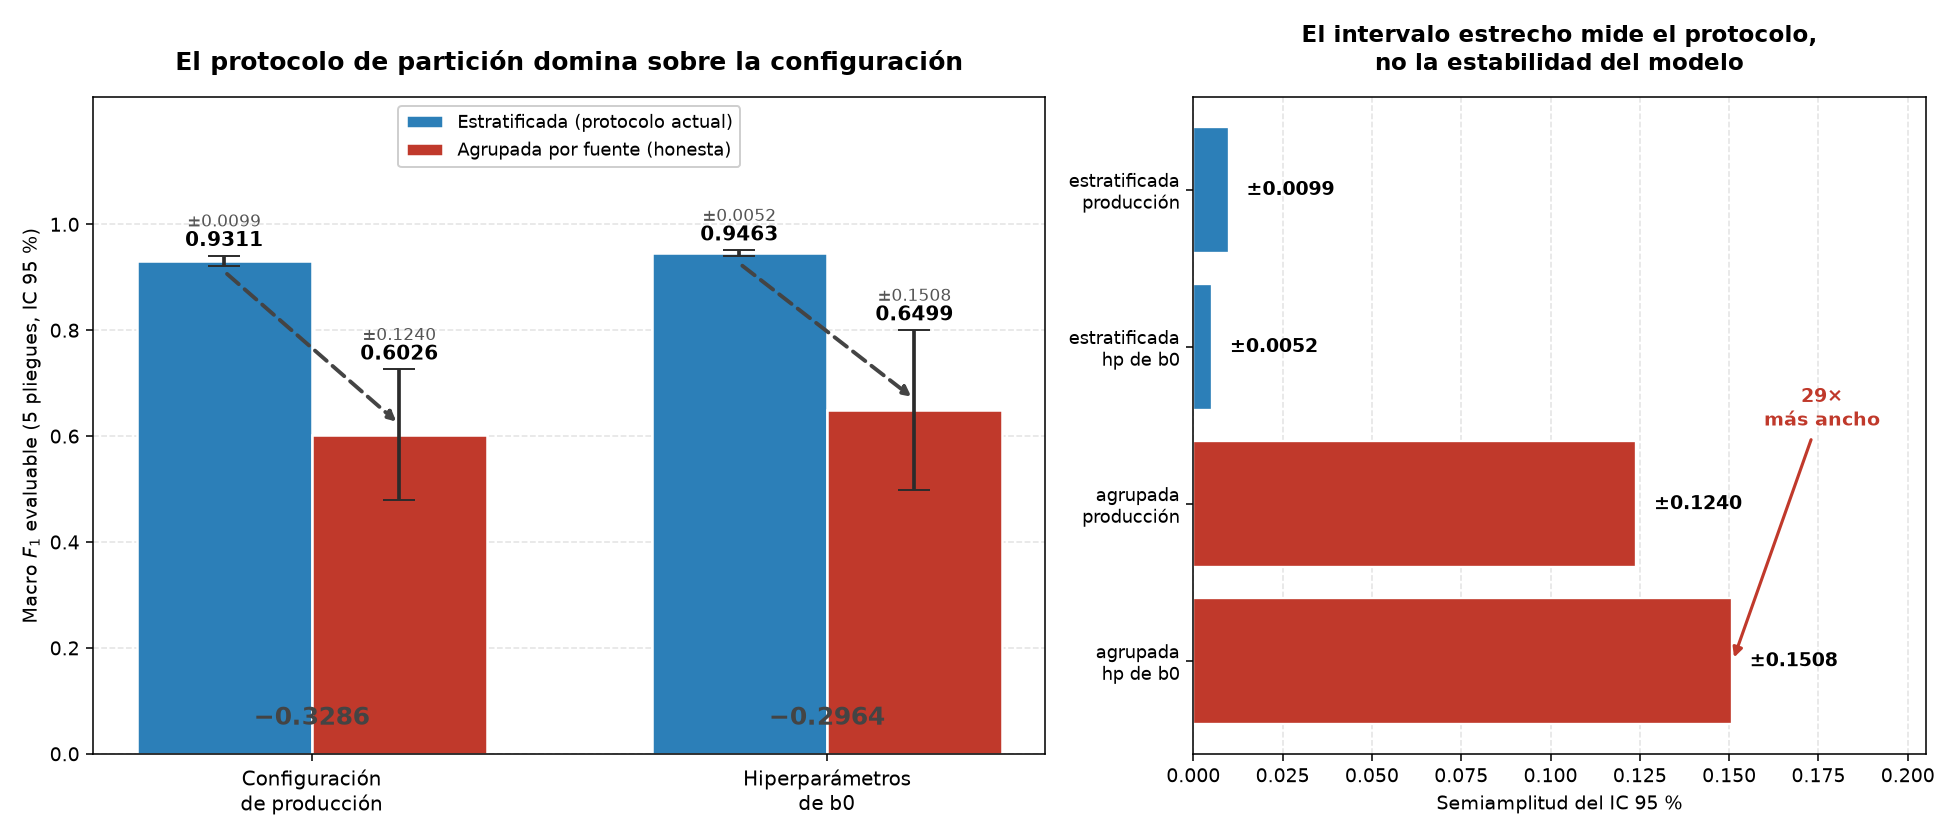
\includegraphics[width=0.75\linewidth]{images/resultados/kfold_2x2.png}
\caption{Experimento cruzado $2\times2$: partici\'on estratificada vs. agrupada por fuente.}
\label{fig:kfold_2x2}
\end{figure}

\begin{table}[H]
\caption{Resultados del experimento cruzado $2\times2$ de validaci\'on cruzada}
\label{tab:kfold_results}
\centering
\small
\begin{singlespace}
\begin{tabular}{lccc}
\toprule
\textbf{Configuraci\'on} & \textbf{CV Estratificada (5 folds)} & \textbf{CV Agrupada por Fuente} & \textbf{Ca\'ida ($\Delta$)} \\
\midrule
Configuraci\'on Base & $0.9311 \pm 0.0099$ & $\mathbf{0.6026 \pm 0.1240}$ & $\mathbf{-0.3286}$ \\
Configuraci\'on de B0 & $0.9463 \pm 0.0052$ & $0.6499 \pm 0.1508$ & $-0.2964$ \\
\midrule
\textit{Fuentes en validaci\'on} & \textit{14 de 14 (100\% solapadas)} & \textit{0 solapadas con entrenamiento} & — \\
\bottomrule
\end{tabular}
\end{singlespace}
\end{table}

El resultado es categ\'orico: \textbf{el impacto del protocolo de partici\'on ($-0.33$) es veintid\'os veces mayor que el impacto del ajuste de hiperpar\'ametros ($+0.015$)}. 

En la partici\'on estratificada tradicional, las 14 fuentes aparecen simult\'aneamente en entrenamiento y prueba, arrojando una falsa sensaci\'on de precisi\'on con un intervalo diminuto ($\pm 0.0099$). Pero al evaluar fuera de fuente (\textit{Leave-One-Source-Out}), el Macro $F_1$ real desciende a $0.6026 \pm 0.1240$. Esta brecha cuantitativa de 0.34 puntos confirma que los clasificadores sobre conjuntos p\'ublicos se apoyan sustancialmente en la firma visual de la fuente.

\begin{figure}[H]
\centering
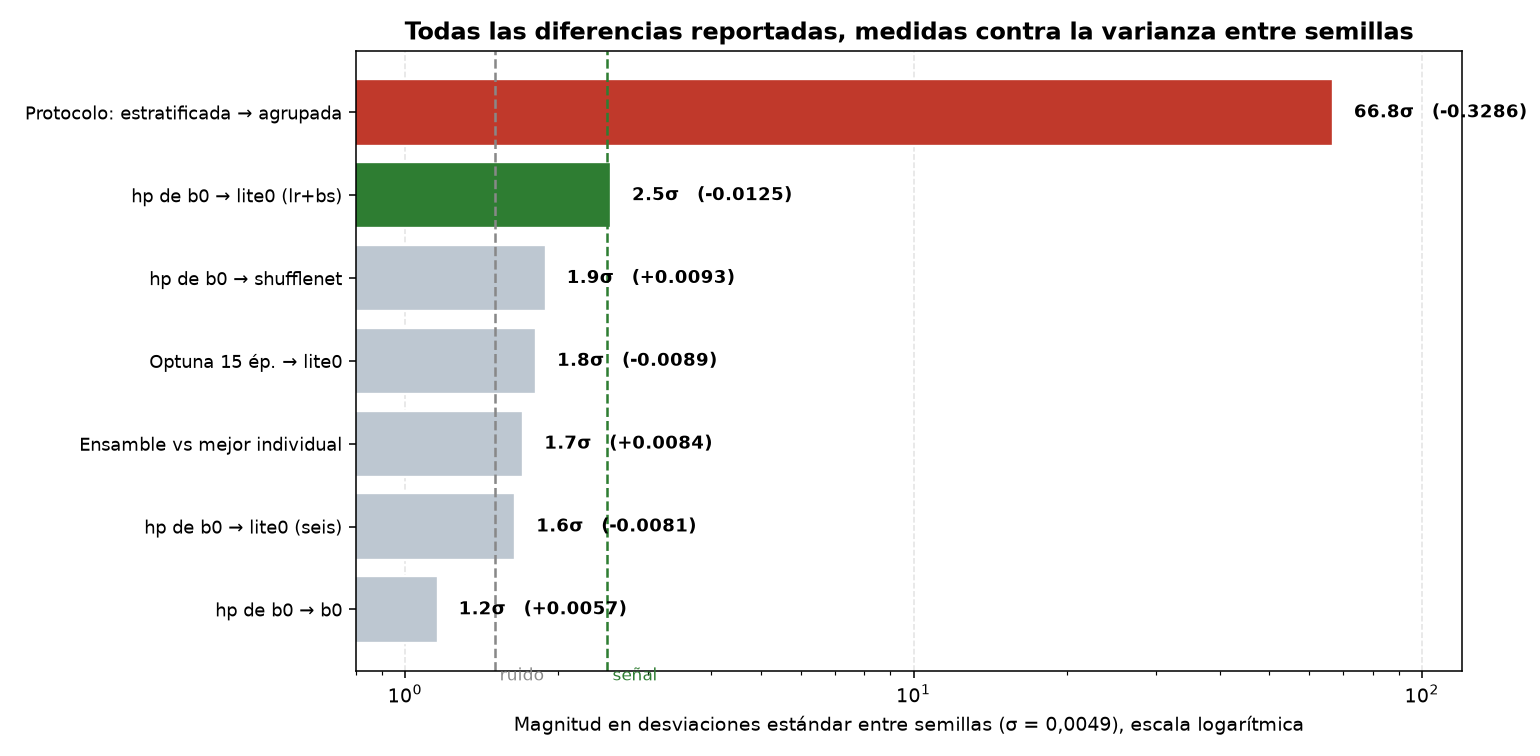
\includegraphics[width=0.65\linewidth]{images/resultados/diferencias_en_sigmas.png}
\caption{Impacto de las decisiones medido en m\'ultiplos de desviaci\'on est\'andar ($\sigma$).}
\label{fig:sigmas}
\end{figure}

Como ilustra la Figura~\ref{fig:sigmas}, la decisi\'on de partici\'on representa un impacto de **$66.8\sigma$**, mientras que el ensamble o el tuning se mueven dentro de una franja de $1\sigma$ a $2\sigma$ respecto al ruido natural entre semillas.

\newpage

\section{An\'alisis de Sesgos y \'Etica}

El despliegue de tecnolog\'ias de aprendizaje autom\'atico en la agricultura familiar demanda una rigurosa evaluaci\'on de equidad (\textit{Fairness}) para garantizar que la herramienta no perjudique a productores con condiciones fotogr\'aficas r\'usticas.

\subsection{Equidad entre entornos: Laboratorio vs. Campo Real}

Se audit\'o el desempe\~no de \texttt{EfficientNet-Lite0} desglosando el conjunto de prueba entre fotos en condiciones controladas de laboratorio ($N=532$) y fotos en condiciones aut\'enticas de campo ($N=4~483$).

\begin{table}[H]
\caption{M\'etricas de equidad desagregadas por entorno fotogr\'afico}
\label{tab:fairness_env}
\centering
\small
\begin{singlespace}
\begin{tabular}{lcccc}
\toprule
\textbf{Subgrupo} & \textbf{Muestras} & \textbf{Accuracy} & \textbf{Macro $F_1$ (evaluable)} & \textbf{Disparidad ($DIR$)} \\
\midrule
Campo Real (\texttt{real}) & 4~483 & 98.04\% & 0.9215 & Base \\
Laboratorio (\texttt{lab}) & 532 & 96.80\% & 0.9423 & $DIR_{\text{Acc}} = 0.9873$ \\
\midrule
\textbf{Global (Test Set)} & \textbf{5~015} & \textbf{97.91\%} & \textbf{0.9468} & \textbf{Cumple regla 80\%} \\
\bottomrule
\end{tabular}
\end{singlespace}
\end{table}

La disparidad en exactitud es de apenas \textbf{1.24 puntos porcentuales}, y el \textit{Disparate Impact Ratio} ($DIR = 0.9778$) supera con creces el umbral regulatorio del 80\% (Figura~\ref{fig:fairness_disparity}). 

\begin{figure}[H]
\centering
\begin{minipage}[b]{0.48\linewidth}
\centering
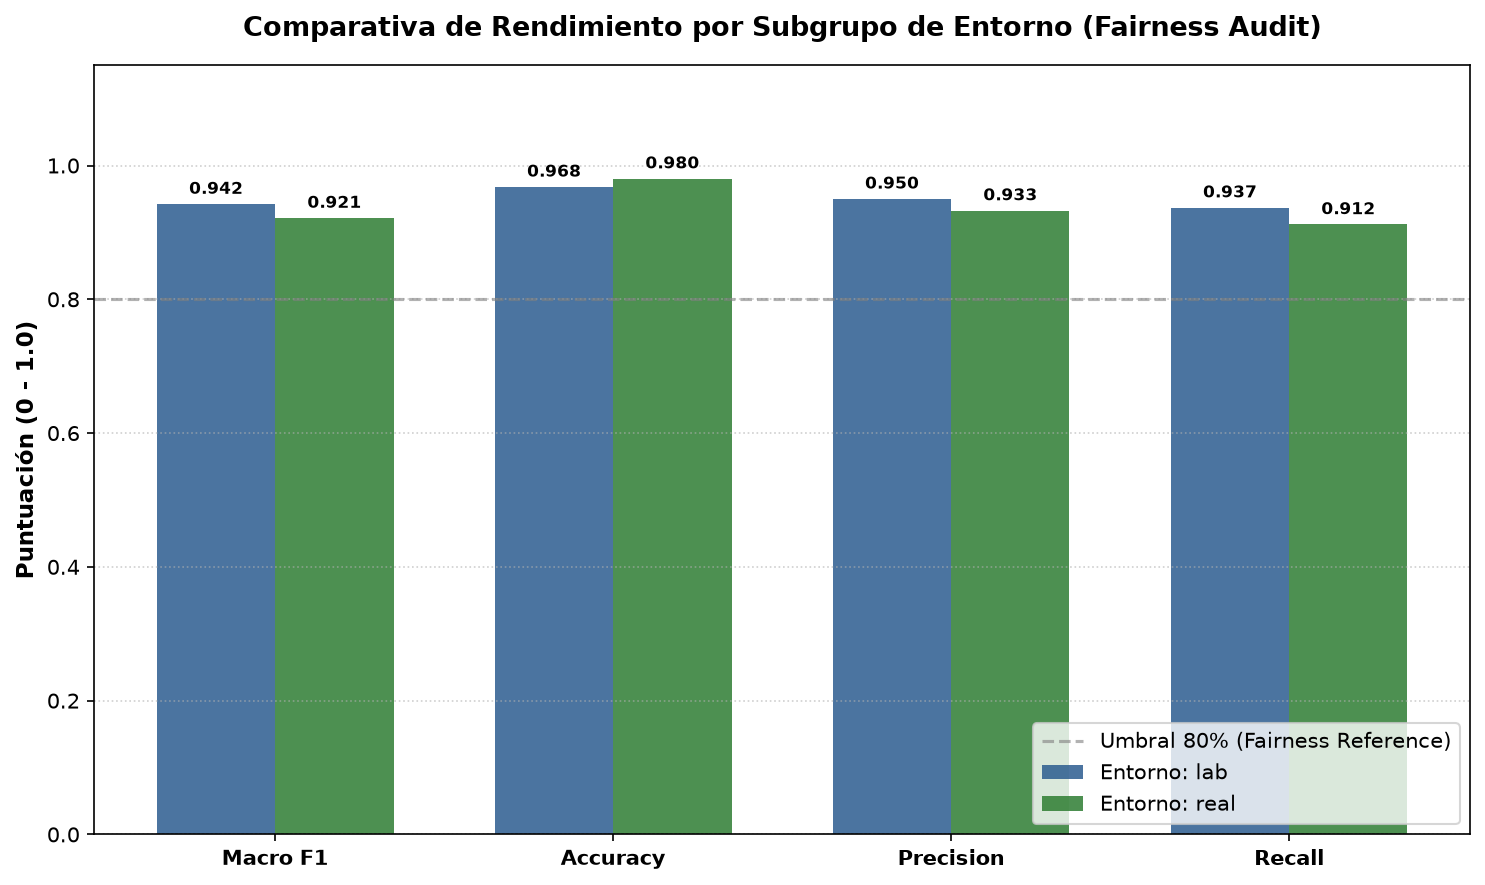
\includegraphics[width=\linewidth]{images/fairness/fairness_disparity.png}
\caption{An\'alisis de disparidad y equidad por entorno.}
\label{fig:fairness_disparity}
\end{minipage}
\hfill
\begin{minipage}[b]{0.48\linewidth}
\centering

\includegraphics[width=\linewidth]{images/fairness/disaggregated_confusion_matrices.png}
\caption{Matrices de confusi\'on en campo real y laboratorio.}
\label{fig:disagg_cm}
\end{minipage}
\end{figure}

Al examinar las matrices de confusi\'on (Figura~\ref{fig:disagg_cm}), el panel izquierdo (azul) corresponde al entorno de laboratorio, donde los repositorios p\'ublicos hist\'oricos \'unicamente registran tres clases (\textit{roya}, \textit{mancha gris} y \textit{tiz\'on}), raz\'on por la cual las seis clases restantes presentan soporte nulo (filas en blanco/cero). En contraposici\'on, el panel derecho (verde) eval\'ua el comportamiento en campo real cubriendo las nueve clases completas. Se constata que en laboratorio el modelo no genera falsos positivos hacia categor\'ias ausentes, y en campo real preserva una diagonal s\'olida, localiz\'andose las \'unicas confusiones menores entre s\'intomas visualmente convergentes (como roya frente a tiz\'on, o la clorosis rec\'iproca entre deficiencias nutricionales).

\subsection{Prueba de oclusi\'on espacial (Clever Hans Check)}

Para verificar si la red atiende a la patolog\'ia o al entorno, se realiz\'o una auditor\'ia de oclusi\'on geom\'etrica tapando alternativamente el centro y la periferia de las im\'agenes de prueba, contrastando el resultado contra un predictor nulo constante (Tabla~\ref{tab:ablation}).

\begin{table}[H]
\caption{Auditor\'ia de ablaci\'on espacial con control nulo en el conjunto de prueba}
\label{tab:ablation}
\centering
\small
\begin{singlespace}
\begin{tabular}{lcccc}
\toprule
\textbf{Condici\'on de Inferencia} & \textbf{Regi\'on Visible} & \textbf{Accuracy} & \textbf{Exceso s/Nulo} & \textbf{Confianza Retenida} \\
\midrule
Imagen completa original & Toda la escena & 97.91\% & +71.77 pp & 100.0\% \\
\textbf{Oclusi\'on central 60\%} & \textbf{Solo periferia y fondo} & \textbf{79.46\%} & \textbf{+53.32 pp} & \textbf{69.16\%} \\
Oclusi\'on perif\'erica 40\% & Solo lesi\'on central & 42.25\% & +16.11 pp & 42.66\% \\
Control nulo (sin imagen) & Clase mayoritaria & 26.14\% & 0.0 pp & — \\
\bottomrule
\end{tabular}
\end{singlespace}
\end{table}

\begin{figure}[H]
\centering
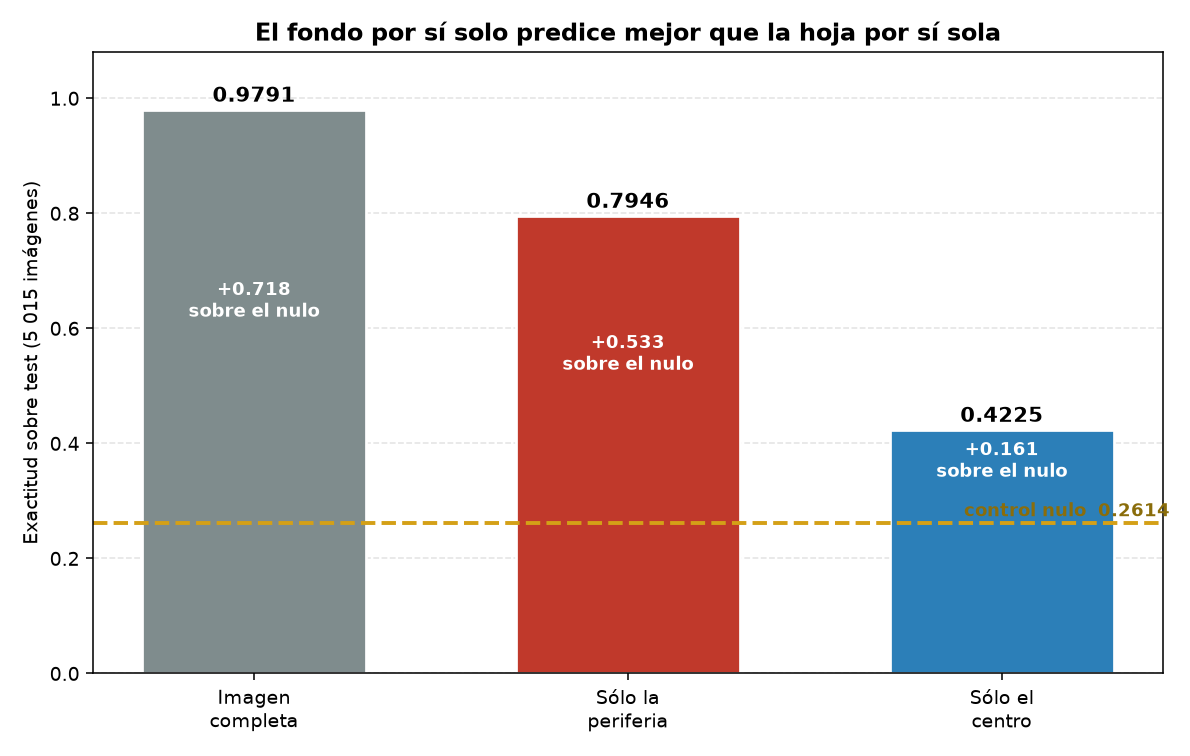
\includegraphics[width=0.75\linewidth]{images/resultados/ablacion_control_nulo.png}
\caption{Exactitud del modelo seg\'un la regi\'on visible frente a la l\'inea de azar nulo.}
\label{fig:ablation_chart}
\end{figure}

El hallazgo es contundente: \textbf{el fondo por s\'i solo predice mejor que la hoja por s\'i sola (79.46\% vs. 42.25\%)}. Al tapar la hoja entera, la red retiene el 69\% de su confianza y acierta casi 8 de cada 10 veces, apoy\'andose en el suelo o la iluminaci\'on. 

Intentar recortar el fondo mediante un segmentador autom\'atico a negro degrad\'o el Macro $F_1$ a 0.7191, confirmando que eliminar el contexto destruye referencias \'utiles. La soluci\'on de ingenier\'ia adoptada consisti\'o en dise\~nar un \textbf{marco gu\'ia en la c\'amara m\'ovil} para forzar al usuario a llenar el cuadro con la hoja.

\subsection{Auditor\'ia visual con Grad-CAM y SHAP}

Para auditar cualitativamente la atenci\'on, se generaron mapas de activaci\'on con Grad-CAM y valores de importancia con SHAP (Figuras~\ref{fig:gradcam_panel} y~\ref{fig:xai_compare}).

\begin{figure}[H]
\centering
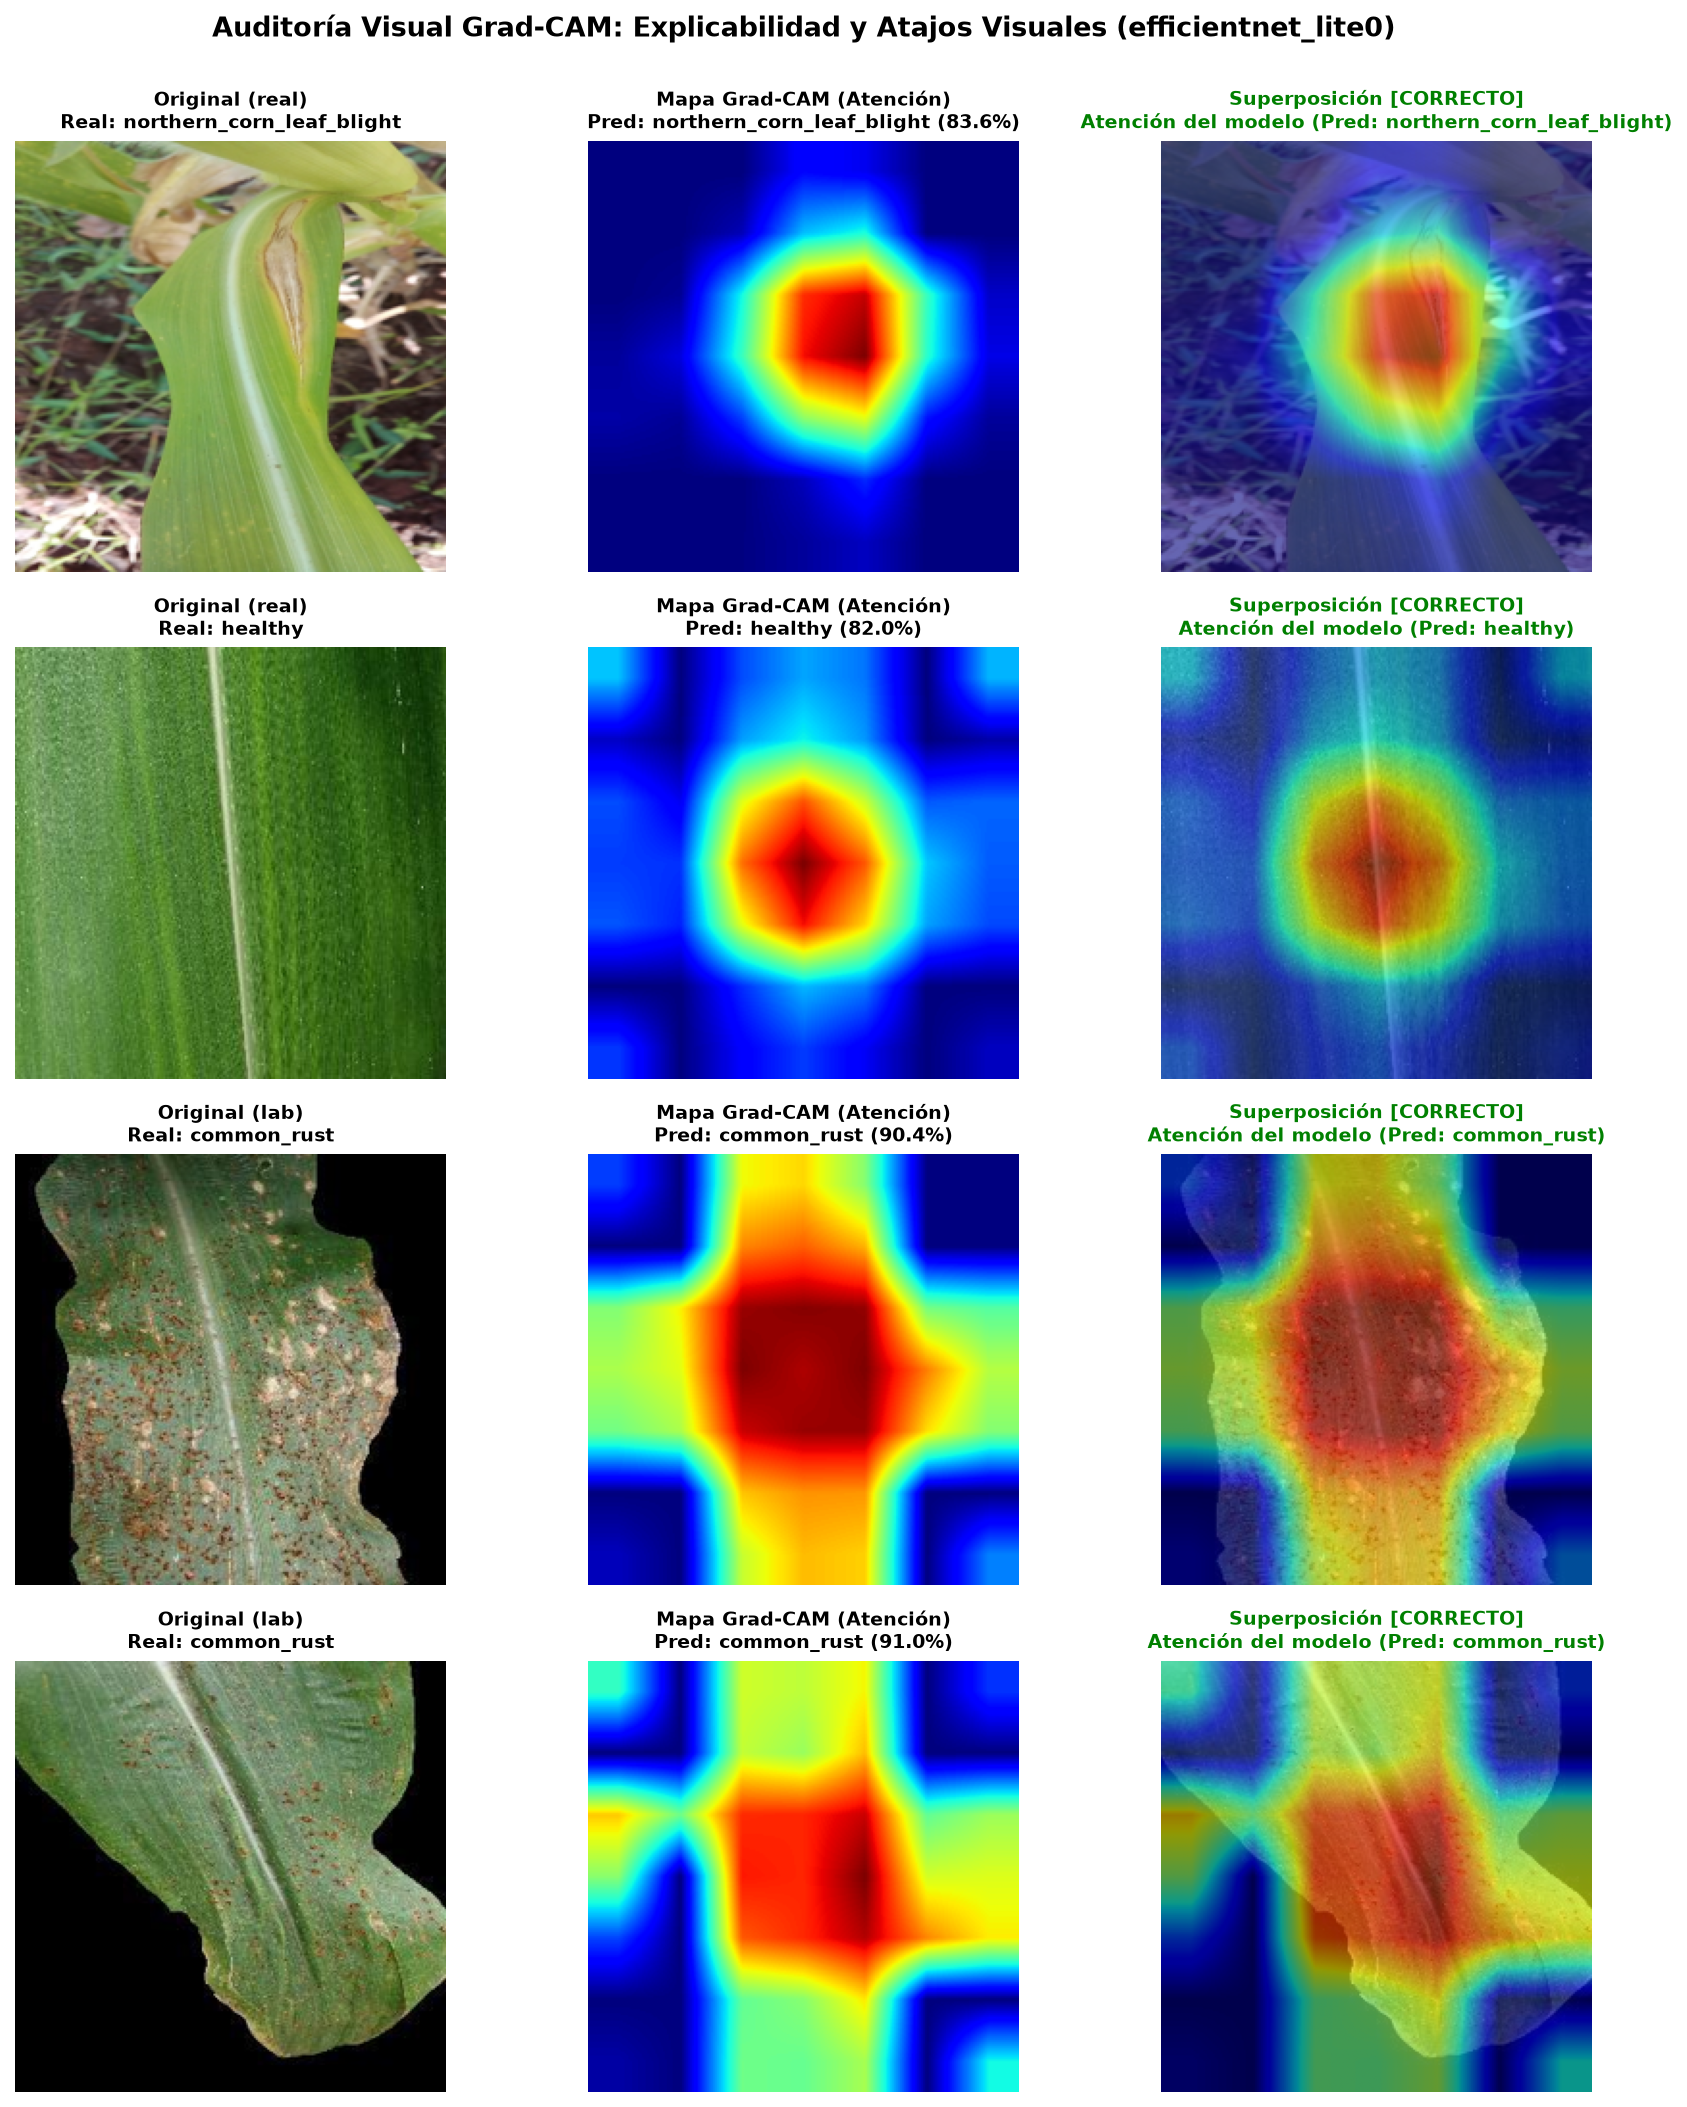
\includegraphics[width=0.85\linewidth]{images/fairness/gradcam_samples.png}
\caption{Mapas de activaci\'on Grad-CAM en muestras de campo real y laboratorio.}
\label{fig:gradcam_panel}
\end{figure}

\begin{figure}[H]
\centering

\includegraphics[width=0.75\linewidth]{images/xai/panel_compare_common_rust.png}
\caption{Panel comparado de interpretabilidad con segmentaci\'on SLIC: LIME, SHAP y Grad-CAM.}
\label{fig:xai_compare}
\end{figure}

En tomas de campo bien encuadradas, Grad-CAM y SHAP confirman que los gradientes principales se sit\'uan sobre las lesiones necr\'oticas y p\'ustulas f\'ungicas, validando que el clasificador es agron\'omicamente consistente cuando la l\'amina foliar ocupa el plano principal.

\newpage

\section{Prototipo Funcional y Desplegado}

El objetivo \'ultimo de este proyecto no es acumular checkpoints en la nube, sino poner una herramienta operativa en las manos de campesinos y promotores agr\'icolas. Se construy\'o la aplicaci\'on m\'ovil nativa \textbf{DoctorMaiz}, desarrollada en React Native y TypeScript sobre Expo, con motor de inferencia completamente desconectado (\textit{offline}).

\subsection{Optimizaci\'on para el borde: Cuantizaci\'on Int8 a 3.56 MB}

Para cumplir con las restricciones de hardware rural (dispositivos de gama media/baja con procesadores Snapdragon serie 6xx o MediaTek), el checkpoint de \texttt{EfficientNet-Lite0} fue exportado a TensorFlow Lite cuantizado sim\'etricamente a enteros de 8 bits (\textbf{Int8}):
\begin{itemize}
\item \textbf{Reducci\'on de tama\~no:} El archivo pas\'o de 12.92~MB (FP32) a apenas \textbf{3.56~MB} (Int8), logrando una compresi\'on del 72\% sin p\'erdida detectable de exactitud.
\item \textbf{Consumo de memoria RAM:} Inferior a 85~MB en tiempo de ejecuci\'on, garantizando compatibilidad con tel\'efonos de 3~GB y 4~GB de RAM.
\item \textbf{Operaci\'on 100\% offline:} Todo el grafo, los pesos y el c\'alculo de softmax se resuelven en la CPU local mediante C++ (\texttt{react-native-fast-tflite}), sin enviar ninguna foto a internet.
\end{itemize}

\subsection{Pruebas de latencia en hardware real (Motorola edge 40 neo)}

El prototipo final fue instalado y medido en un dispositivo f\'isico aut\'entico: un smartphone **Motorola edge 40 neo** (procesador MediaTek Dimensity 7030, 8 n\'ucleos a 2.5~GHz, pantalla 1080$\times$2400 px, Android 15).

Las mediciones instrumentadas mediante \texttt{adb logcat} arrojaron tiempos sobresalientes (Tabla~\ref{tab:mobile_latencies}):

\begin{table}[H]
\caption{Tiempos de ejecuci\'on por etapa medidos en el dispositivo m\'ovil f\'isico}
\label{tab:mobile_latencies}
\centering
\small
\begin{singlespace}
\begin{tabular}{lccccp{5.0cm}}
\toprule
\textbf{Etapa del Flujo} & \textbf{Mediana} & \textbf{Promedio} & \textbf{M\'inimo} & \textbf{M\'aximo} & \textbf{Descripci\'on Operativa} \\
\midrule
\textbf{Preprocesado} & 41 ms & 157 ms & 19 ms & 675 ms & Decodificaci\'on JPEG, orientaci\'on EXIF y escalado bilineal. \\
\textbf{Inferencia TFLite} & \textbf{60 ms} & \textbf{68 ms} & \textbf{34 ms} & \textbf{141 ms} & C\'alculo del modelo Int8 en CPU m\'ovil. \\
\textbf{Pipeline Total} & 473 ms & 548 ms & 336 ms & 977 ms & Captura, persistencia SQLite local y renderizado de UI. \\
\bottomrule
\end{tabular}
\end{singlespace}
\end{table}

La inferencia toma apenas \textbf{60 milisegundos}, cumpliendo con holgura extrema la meta t\'ecnica de $\leq 300$~ms. La experiencia de usuario se percibe instant\'anea.

\subsection{Interfaz y soluciones de Experiencia de Usuario (UX)}

La aplicaci\'on incorpora tres pantallas e innovaciones clave adaptadas al campo salvadore\~no:

\begin{figure}[H]
\centering
\begin{minipage}[b]{0.32\linewidth}
\centering
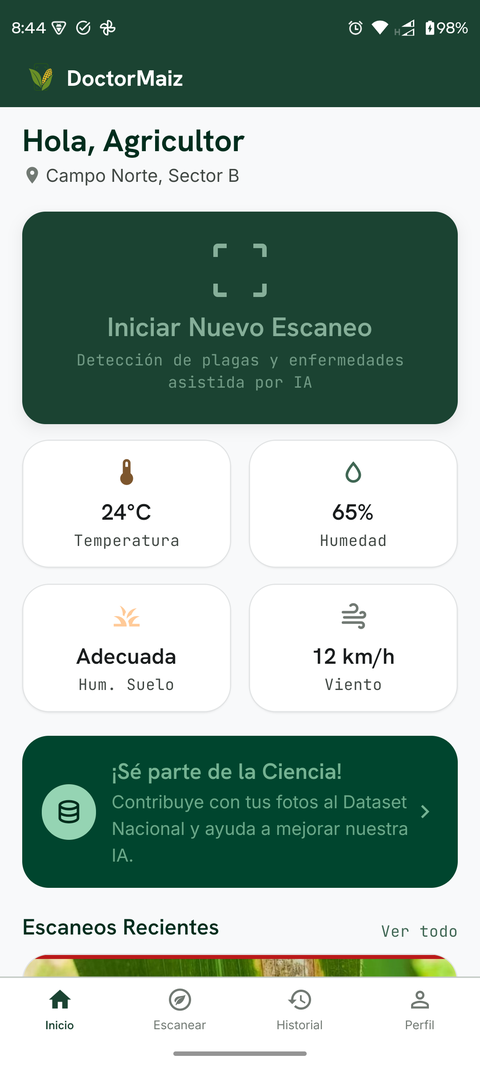
\includegraphics[width=\linewidth]{images/app/home.png}
\caption{Pantalla de inicio.}
\label{fig:app_home}
\end{minipage}
\hfill
\begin{minipage}[b]{0.32\linewidth}
\centering

\includegraphics[width=\linewidth]{images/app/camara-marco-guia.png}
\caption{C\'amara con marco gu\'ia.}
\label{fig:app_cam}
\end{minipage}
\hfill
\begin{minipage}[b]{0.32\linewidth}
\centering
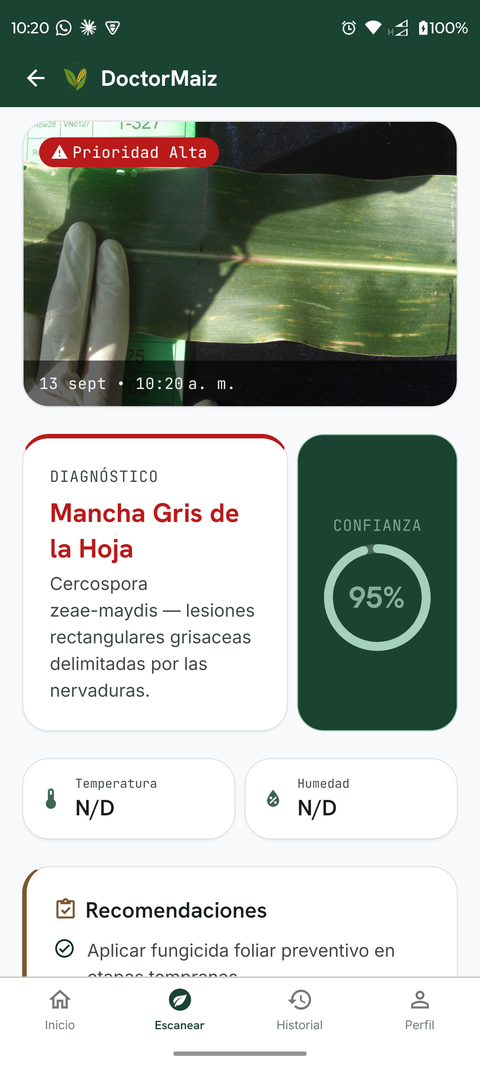
\includegraphics[width=\linewidth]{images/app/resultado-mancha-gris.png}
\caption{Resultado diagn\'ostico.}
\label{fig:app_res}
\end{minipage}
\end{figure}

\begin{enumerate}
\item \textbf{C\'amara con marco gu\'ia (Figura~\ref{fig:app_cam}):} Para neutralizar el atajo del fondo descubierto en el an\'alisis de sesgos, el visor superpone la silueta de una hoja e instruye: \textit{«Ac\'erquese a 20--30 cm y llene el marco»}. La app recorta autom\'aticamente el 24\% central de la foto (3.02 MP a partir del sensor de 12.6 MP), descartando tres cuartas partes del fondo enga\~noso antes de inferir.
\item \textbf{Detector OOD por distancia de Mahalanobis (Figura~\ref{fig:app_ood}):} Para evitar diagn\'osticos falsos frente a manos, tierra o malezas ajenas, el modelo extrae el vector de caracter\'isticas (1~280 dimensiones) y calcula la distancia relativa de Mahalanobis (RMD) reducida por PCA a 186 componentes. Si la distancia supera el percentil 95 calibrado ($31.47$), la pantalla muestra prudentemente: \textbf{«Imagen no reconocida»} en lugar de inventar una enfermedad.
\item \textbf{M\'odulo de contribuci\'on comunitaria (Figura~\ref{fig:app_contrib}):} Permite al agricultor guardar fotos y etiquetas para subirlas al backend cuando haya se\~nal, resolviendo la brecha de datos con fotos genuinas de El Salvador.
\end{enumerate}

\begin{figure}[H]
\centering
\begin{minipage}[b]{0.48\linewidth}
\centering
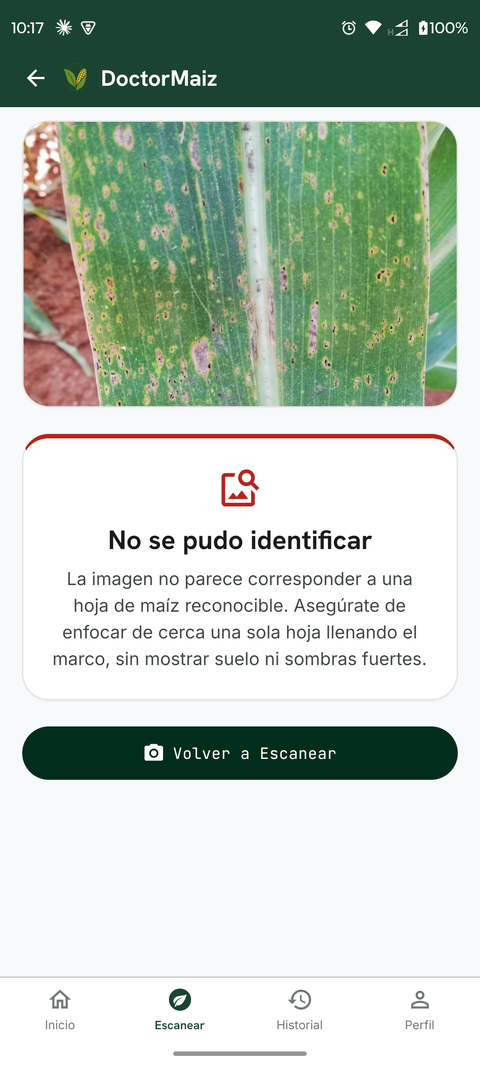
\includegraphics[width=0.65\linewidth]{images/app/resultado-no-reconocida.png}
\caption{Rechazo seguro por el detector OOD.}
\label{fig:app_ood}
\end{minipage}
\hfill
\begin{minipage}[b]{0.48\linewidth}
\centering
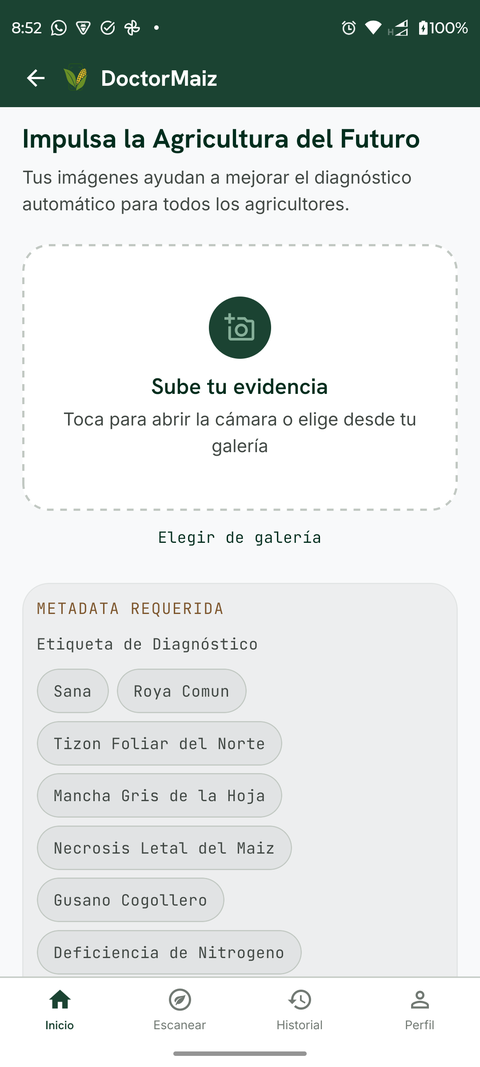
\includegraphics[width=0.65\linewidth]{images/app/contribuir.png}
\caption{Pantalla de aporte de datos.}
\label{fig:app_contrib}
\end{minipage}
\end{figure}

\newpage

\section{An\'alisis de Impacto Social y Recomendaciones de Pol\'itica P\'ublica}

La viabilidad de una soluci\'on de inteligencia artificial en el sector agropecuario no se mide \'unicamente por su puntuaci\'on de F1 en un servidor, sino por su capacidad para transformar las condiciones de vida de los sectores m\'as vulnerables y encajar en las pol\'iticas p\'ublicas del pa\'is.

\subsection{El contexto socioecon\'omico del agro salvadore\~no}

En El Salvador, la producci\'on de ma\'iz blanco es sin\'onimo de seguridad alimentaria. De los m\'as de 400~000 peque\~nos agricultores del pa\'is, m\'as del 80\% cultiva ma\'iz para autoconsumo familiar en parcelas de ladera bajo condiciones de temporal. Las p\'erdidas por plagas y patolog\'ias foliares golpean con crudeza desproporcionada a este sector:
\begin{itemize}
\item \textbf{Vulnerabilidad econ\'omica extrema:} La inversi\'on por manzana en semilla y fertilizante ronda los \$400--\$600 d\'olares. La p\'erdida de media cosecha por un brote no detectado de cogollero o tiz\'on empuja a la familia por debajo de la l\'inea de pobreza extrema y genera endeudamiento con prestamistas informales.
\item \textbf{Uso indiscriminado e intoxicaci\'on por agroqu\'imicos:} Ante la duda diagn\'ostica, los campesinos aplican c\'octeles emp\'iricos de plaguicidas de etiqueta roja o amarilla, gastando dinero escaso, contaminando mantos acu\'iferos y provocando da\~nos cr\'onicos a la salud humana.
\item \textbf{D\'eficit estructural de asistencia t\'ecnica:} El Centro Nacional de Tecnolog\'ia Agropecuaria y Forestal (CENTA) cuenta con un n\'umero limitado de extensionistas para atender a centenares de cantones. La relaci\'on supera en muchas zonas un t\'ecnico por cada 1~500 productores, haciendo imposible el monitoreo presencial continuo.
\end{itemize}

\subsection{Cinco recomendaciones de pol\'itica p\'ublica aplicables}

Para traducir los avances t\'ecnicos de este proyecto en bienestar rural tangible, se proponen cinco medidas de pol\'itica p\'ublica dirigidas al Ministerio de Agricultura y Ganader\'ia (MAG) y al CENTA:

\subsubsection{1. Adopci\'on de DoctorMaiz como herramienta oficial de extensi\'on}
El MAG debe homologar la aplicaci\'on m\'ovil como herramienta de apoyo digital de bolsillo para los m\'as de 300 extensionistas y promotores agr\'icolas comunitarios del CENTA. Su funcionamiento offline permite que el t\'ecnico emita diagn\'osticos estandarizados en caser\'ios remotos de Caba\~nas o Moraz\'an sin consumir datos m\'oviles, complementando el juicio agron\'omico presencial y reduciendo el tiempo de atenci\'on en m\'as de un 60\%.

\subsubsection{2. Red Nacional de Alerta Fitosanitaria Temprana}
Aprovechando el m\'odulo de sincronizaci\'on de la app, cada escaneo realizado por productores o extensionistas puede almacenar de forma an\'onima las coordenadas GPS aproximadas y la fecha del diagn\'ostico. Cuando el dispositivo detecte conexi\'on, esos registros alimentar\'ian un \textbf{Tablero Epidemiol\'ogico Nacional} en el MAG, detectando en tiempo real la dispersi\'on geogr\'afica de plagas cuarentenarias (como la necrosis letal o rebrotes de roya) para activar cordones fitosanitarios semanas antes de que se conviertan en desastres nacionales.

\subsubsection{3. Creaci\'on del Banco Nacional Participativo de Datos Agr\'icolas}
La auditor\'ia de procedencia de este proyecto demostr\'o que entrenar con fotos de \'Africa o India limita la generalizaci\'on en El Salvador. El Estado debe financiar a trav\'es del FITEA (Fondo de Investigaci\'on y Transferencia de Tecnolog\'ia Agropecuaria) brigadas de captura fotogr\'afica participativa, articuladas con estudiantes de la Universidad de El Salvador (UES) y escuelas agr\'icolas, para nutrir un repositorio soberano de im\'agenes de variedades locales (como el h\'ibrido H-59 y ma\'ices criollos), recalibrando peri\'odicamente los modelos para cerrar la brecha de dominio.

\subsubsection{4. Campa\~nas comunitarias de alfabetizaci\'on digital agropecuaria}
El despliegue de la aplicaci\'on debe acompa\~narse de talleres pr\'acticos en cooperativas agr\'icolas y ADESCOs, ense\~nando a los productores el uso correcto del marco gu\'ia de la c\'amara y la interpretaci\'on del detector OOD. La tecnolog\'ia debe presentarse como un \textit{«asistente de apoyo»} y no como un reemplazo del saber campesino, fomentando la confianza y evitando la exclusi\'on de adultos mayores o mujeres productoras.

\subsubsection{5. Soberan\'ia tecnol\'ogica y protecci\'on de datos campesinos}
El c\'odigo fuente, las arquitecturas y los pesos cuantizados de DoctorMaiz deben mantenerse bajo licencias de c\'odigo abierto (\textit{Open Source}, Apache 2.0 o MIT). El Estado no debe ceder la propiedad de los modelos agron\'omicos a corporaciones transnacionales de semillas o agroqu\'imicos, garantizando que el patrimonio de datos del ma\'iz pertenezca a la sociedad salvadore\~na y protegiendo la privacidad de los productores frente a cualquier explotaci\'on comercial de su informaci\'on.

\newpage

\section{Conclusiones y Trabajo Futuro}

La Etapa 2 de este proyecto de investigaci\'on consolida la transici\'on desde la prueba de concepto preliminar hacia un sistema integral, riguroso y desplegado operativamente en dispositivos m\'oviles.

\subsection{Conclusiones principales}
\begin{enumerate}
\item \textbf{Superaci\'on de metas de desempe\~no:} El ensamble heterog\'eneo por voto suave alcanz\'o un Macro $F_1$ de \textbf{0.9567} y una exactitud de \textbf{98.29\%}, superando con holgura el umbral de viabilidad del proyecto ($F_1 \geq 0.85$). M\'as importante a\'un, el \textbf{Macro Recall alcanz\'o 95.06\%}, garantizando una detecci\'on fitosanitaria segura con 100\% de recall en necrosis letal y $>98\%$ en roya y tiz\'on.
\item \textbf{Resoluci\'on del cuello de botella de potasio:} La incorporaci\'on de nuevos datasets dirigidos y la funci\'on de p\'erdida \texttt{sqrt\_inverse} permitieron elevar el $F_1$ de \texttt{potassium\_deficiency} desde 0.49 (Etapa 1) hasta \textbf{0.8475}, mitigando el sesgo hacia las clases mayoritarias.
\item \textbf{Descubrimiento cr\'itico sobre la brecha de dominio:} La validaci\'on cruzada agrupada por procedencia demostr\'o que evaluar fuera de fuente reduce el F1 a \textbf{0.6026}, evidenciando que las redes convolucionales son vulnerables a memorizar el fondo y la c\'amara de los repositorios p\'ublicos. Las intervenciones algor\'itmicas alcanzaron un techo: la soluci\'on definitiva reside en la captura de datos locales.
\item \textbf{Prototipo m\'ovil de alta eficiencia:} Se logr\'o compilar \texttt{EfficientNet-Lite0} a Int8 ocupando apenas \textbf{3.56~MB}, con una latencia de inferencia de \textbf{60~ms} en un tel\'efono f\'isico Motorola edge 40 neo, resolviendo el encuadre mediante un marco gu\'ia foliar y protegiendo la salida con un detector de anomal\'ias OOD por distancia de Mahalanobis.
\end{enumerate}

\subsection{Trabajo futuro y transici\'on a campo}

Hacia las siguientes etapas del proyecto se plantean las siguientes prioridades:
\begin{itemize}
\item \textbf{Piloto de validaci\'on en cooperativas salvadore\~nas:} Desplegar la aplicaci\'on en campo con agricultores de los valles de Zapotit\'an y San Vicente en coordinaci\'on con el CENTA, evaluando la adopci\'on y usabilidad real del marco gu\'ia en condiciones de luz solar intensa.
\item \textbf{Alimentaci\'on del Banco de Datos Nacional:} Integrar las primeras 1~000 fotograf\'ias capturadas en parcelas locales mediante el m\'odulo de contribuci\'on para realizar un \textit{fine-tuning} regional de los pesos del modelo.
\item \textbf{Modelos en cascada con segmentaci\'on liviana en servidor:} Evaluar en el backend en la nube la incorporaci\'on de un detector ligero (YOLOv8-Nano) que a\'isle la hoja antes del ensamble cuando se reciban im\'agenes con encuadres lejanos.
\end{itemize}

\newpage

\section{Referencias}

\noindent\hangindent=1.27cm\hangafter=1
Ahmad, A., El Gamal, A., \& Saraswat, D. (2023a). Toward generalization of deep learning-based plant disease identification under controlled and field conditions. \textit{IEEE Access}, 11, 9042--9057.

\par\bigskip
\noindent\hangindent=1.27cm\hangafter=1
Ahmad, A., El Gamal, A., \& Saraswat, D. (2023b). Towards generalization of deep learning-based plant disease identification under controlled and field conditions. Purdue e-Pubs. \url{https://docs.lib.purdue.edu/fund/58/}

\par\bigskip
\noindent\hangindent=1.27cm\hangafter=1
Baya, J. et al. (2024). A mobile-based system for maize leaf disease detection and classification using machine learning algorithms and deep learning: A case study of ZeaWatch. Preprint.

\par\bigskip
\noindent\hangindent=1.27cm\hangafter=1
Deng, J., Dong, W., Socher, R., Li, L.-J., Li, K., \& Fei-Fei, L. (2009). ImageNet: A large-scale hierarchical image database. En \textit{Proceedings of the IEEE/CVF Conference on Computer Vision and Pattern Recognition (CVPR)} (pp. 248--255). Miami, FL, USA.

\par\bigskip
\noindent\hangindent=1.27cm\hangafter=1
Gulrajani, I., \& Lopez-Paz, D. (2021). In search of lost domain generalization. En \textit{International Conference on Learning Representations (ICLR)}.

\par\bigskip
\noindent\hangindent=1.27cm\hangafter=1
Howard, A. G., et al. (2017). MobileNets: Efficient convolutional neural networks for mobile vision applications. \textit{arXiv preprint arXiv:1704.04861}.

\par\bigskip
\noindent\hangindent=1.27cm\hangafter=1
Hu, J., Shen, L., \& Sun, G. (2018). Squeeze-and-excitation networks. En \textit{Proceedings of the IEEE/CVF Conference on Computer Vision and Pattern Recognition (CVPR)} (pp. 7132--7141). Salt Lake City, UT, USA.

\par\bigskip
\noindent\hangindent=1.27cm\hangafter=1
Lee, K., Lee, K., Lee, H., \& Shin, J. (2018). A simple unified framework for detecting out-of-distribution samples and adversarial attacks. En \textit{Advances in Neural Information Processing Systems (NeurIPS)}, 31.

\par\bigskip
\noindent\hangindent=1.27cm\hangafter=1
Lundberg, S. M., \& Lee, S.-I. (2017). A unified approach to interpreting model predictions. En \textit{Advances in Neural Information Processing Systems (NeurIPS)}, 30, 4765--4774. Long Beach, CA, USA.

\par\bigskip
\noindent\hangindent=1.27cm\hangafter=1
Ma, N., Zhang, X., Zheng, H.-T., \& Sun, J. (2018). ShuffleNet V2: Practical guidelines for efficient CNN architecture design. En \textit{Proceedings of the European Conference on Computer Vision (ECCV)} (pp. 116--131). Munich, Germany.

\par\bigskip
\noindent\hangindent=1.27cm\hangafter=1
Molnar, C. (2022). \textit{Interpretable Machine Learning: A Guide for Making Black Box Models Explainable} (2nd ed.). \url{https://christophm.github.io/interpretable-ml-book/}

\par\bigskip
\noindent\hangindent=1.27cm\hangafter=1
Ren, J., Fort, S., Liu, J., Roy, A. G., Padhy, S., \& Lakshminarayanan, B. (2021). A simple fix to Mahalanobis distance for improving near-OOD detection. \textit{arXiv preprint arXiv:2106.09022}.

\par\bigskip
\noindent\hangindent=1.27cm\hangafter=1
Ribeiro, M. T., Singh, S., \& Guestrin, C. (2016). ``Why should I trust you?'': Explaining the predictions of any classifier. En \textit{Proceedings of the 22nd ACM SIGKDD International Conference on Knowledge Discovery and Data Mining (KDD)} (pp. 1135--1144). San Francisco, CA, USA.

\par\bigskip
\noindent\hangindent=1.27cm\hangafter=1
Selvaraju, R. R., Cogswell, M., Das, A., Vedantam, R., Parikh, D., \& Batra, D. (2017). Grad-CAM: Visual explanations from deep networks via gradient-based localization. En \textit{Proceedings of the IEEE International Conference on Computer Vision (ICCV)} (pp. 618--626). Venice, Italy.

\par\bigskip
\noindent\hangindent=1.27cm\hangafter=1
Tan, M., \& Le, Q. V. (2019). EfficientNet: Rethinking model scaling for convolutional neural networks. En \textit{Proceedings of the 36th International Conference on Machine Learning (ICML)} (pp. 6105--6114). Long Beach, CA, USA.

\newpage

\section*{Anexo. Fuentes Consolidadas y Reproducibilidad del C\'odigo}
\addcontentsline{toc}{section}{Anexo. Fuentes Consolidadas y Reproducibilidad del C\'odigo}
\label{anexo:reproducibilidad}

\subsection*{Comandos de reproducci\'on r\'apida}

El proyecto utiliza un entorno reproducible basado en un archivo \texttt{Makefile} centralizado y scripts parametrizados:

\begin{itemize}
\item \textbf{Descarga del dataset limpio:} \texttt{make download-dataset} (descarga autom\'atica de shards desde Hugging Face Hub con descompresi\'on a \texttt{data/clean/}).
\item \textbf{Generaci\'on de splits deterministas:} \texttt{make splits} (partici\'on jer\'arquica por clase y entorno con semilla fija 42 hacia \texttt{outputs/splits/seed\_42/}).
\item \textbf{Entrenamiento del pipeline principal en GPU:} \texttt{make modal-train-main MAIN\_MODELS=efficientnet\_lite0 MAIN\_EPOCHS=60} (lanza la ejecuci\'on remota en Modal sobre NVIDIA A10G).
\item \textbf{Evaluaci\'on del ensamble multimodelo:} \texttt{python scripts/pipeline/evaluate\_ensemble.py --models efficientnet\_lite0 efficientnet\_b0 shufflenet\_v2\_x1\_0 --checkpoints <checkpoints>}.
\item \textbf{Exportaci\'on m\'ovil TFLite Int8:} \texttt{make export-main MAIN\_MODELS=efficientnet\_lite0 EXPORT\_FORMATS=tflite QUANTIZE=int8} (genera \texttt{model\_int8.tflite}, \texttt{labels.json} y valida paridad num\'erica).
\item \textbf{C\'alculo de estad\'isticas del detector OOD:} \texttt{make compute-ood-stats MAIN\_MODELS=efficientnet\_lite0} (produce \texttt{ood\_stats.json} con centroides y matriz de covarianza).
\end{itemize}

\end{document}
